\section{Experimental Setup}
\label{sec:setup}

\subsection{Platforms and Software Stack}
\label{subsec:platforms}

The mapping subsystem is implemented as a set of decoupled ROS~2 (Jazzy) nodes.
A mobile base builds a 2D occupancy map online with Cartographer
SLAM~\cite{hess2016}; the frontier explorer~\cite{guler2024} selects goals and
drives the robot through the Nav2 navigation stack~\cite{macenski2020marathon}
using a sampling-based model-predictive path integral
controller~\cite{williams2016}; and the stop-and-scan sequencer applies the
placement policy of Chapter~\ref{ch:mapping}. Nav2 plans on an inflated
costmap, so every path and every scan candidate keeps the robot footprint clear
of obstacles by the inflation margin (0.70~m inflation radius with a 0.22~m
robot radius in all reported runs). The target stationary sensor is a Leica
BLK360~G1 terrestrial laser scanner; a driver connects to the physical device
over Wi-Fi and executes its full-dome scan workflow.

Two mobile platforms are used. \textbf{RedBOT04} (Figure~\ref{fig:redbot}) is
the scan platform: a four-wheeled skid-steer base (footprint $71\times49$~cm)
driven by four BLDC gearmotors, with an industrial PC main controller and an
STM32 sub-controller; a YDLiDAR TG30 provides the 2D scan for SLAM and
navigation, and the BLK360 is mounted on the deck about 0.5~m above the
floor---lower than a typical 1.5--1.8~m tripod setup, so low furniture casts
longer horizontal shadows than in a manual survey. \textbf{AMMR} is the
spatial-operation robot of Chapter~\ref{ch:validation}: a swerve-drive mobile
manipulator (body $1.24\times0.79$~m) running its own AMCL localization and
Nav2 stack on an independently built map. For the controlled coverage
evaluation, a TurtleBot3 Waffle is the mobile base in
Gazebo~\cite{koenig2004gazebo}, and the physical scanner is replaced by a mock
scanner node that reproduces the BLK360 capture-and-download timing and its
failure-and-retry behavior. The semantic modeling pipeline runs on a desktop
workstation (AMD Ryzen~9 9900X, 32~GB RAM, NVIDIA RTX PRO 4000 Blackwell
24~GB), which also hosts Isaac Sim~5.1 for the twin.

\begin{figure}[!htb]
\centering
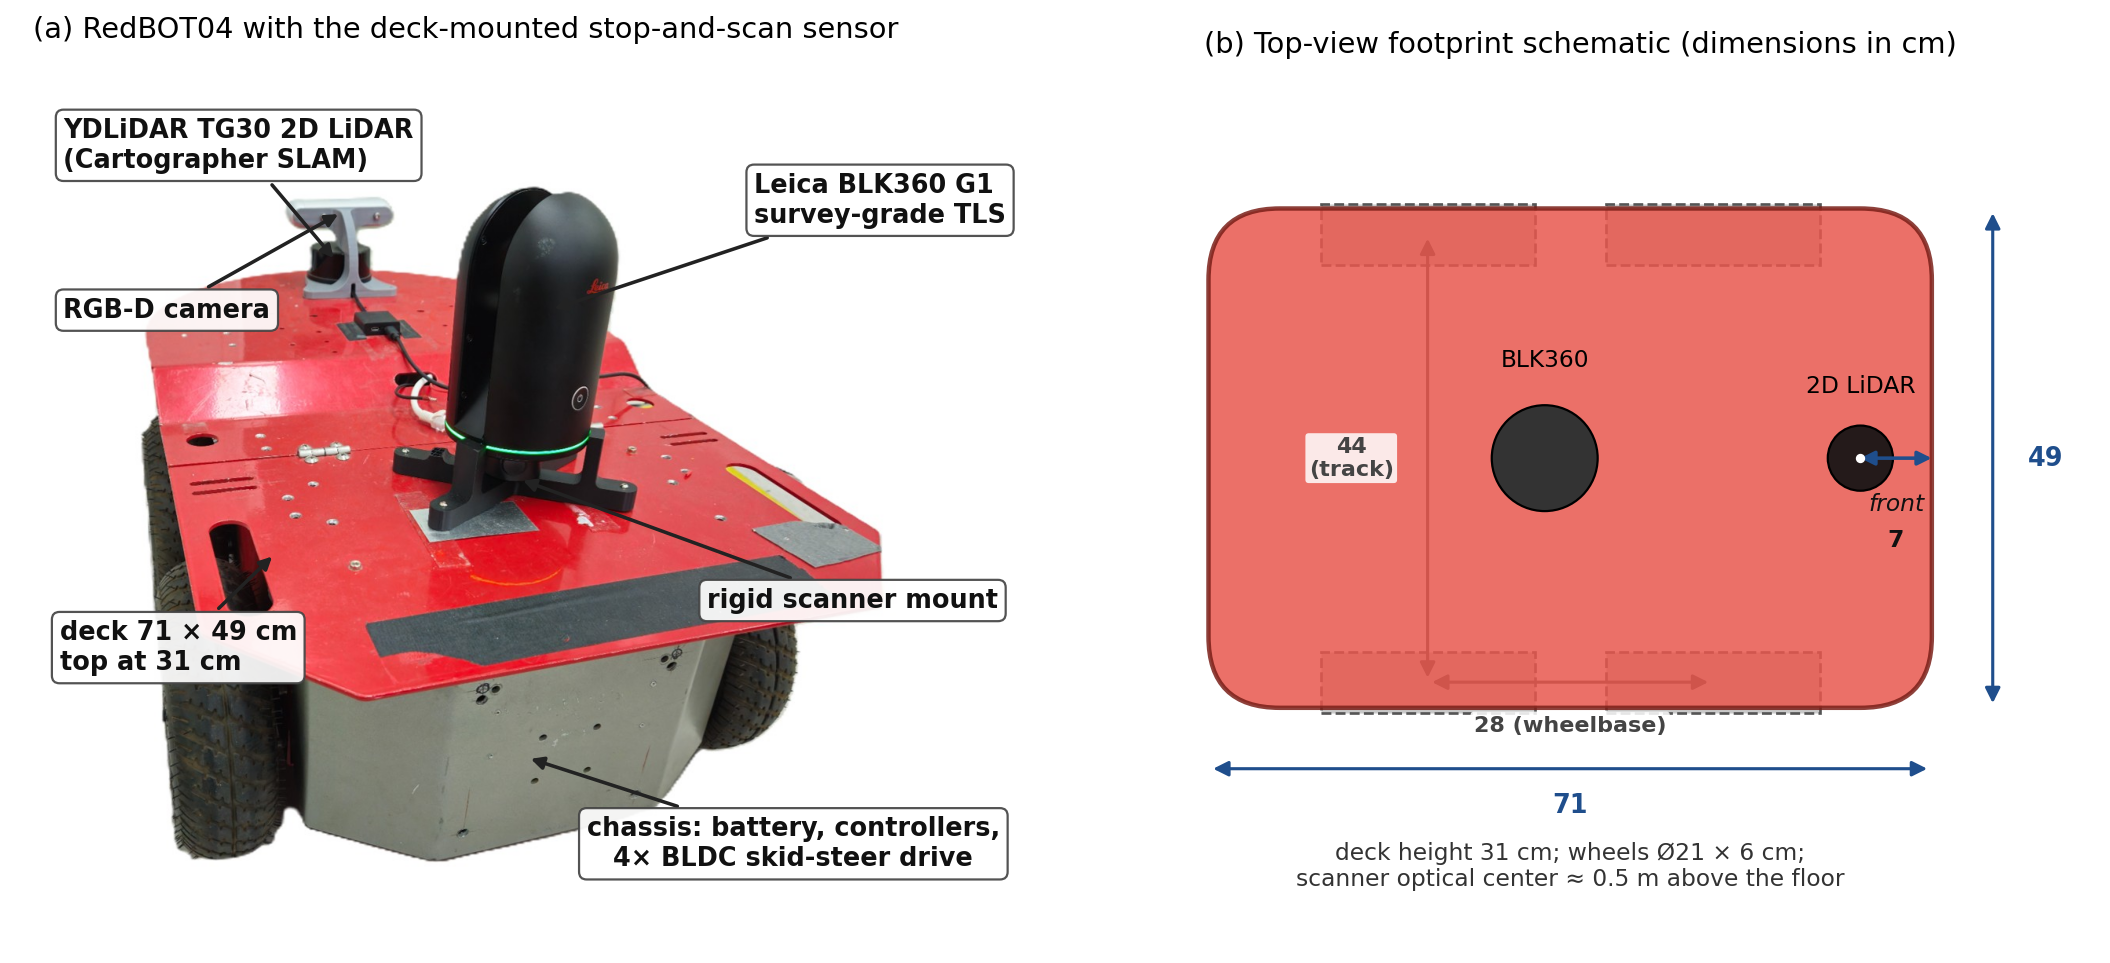
\includegraphics[width=0.9\linewidth]{figures/sen_fig9_redbot04_platform_annot.png}
\caption{RedBOT04 mobile scan platform. (a)~Annotated view with the
deck-mounted Leica BLK360~G1; (b)~top-view footprint schematic with the
principal dimensions (cm).}
\label{fig:redbot}
\end{figure}

\subsection{Environments, Scenes, and Epochs}
\label{subsec:scenes}

Two simulated indoor worlds are used for the mapping ablation. The
single-room world is generated from a real BLK360 scan of the test room,
converted to a 2D occupancy grid and extruded into a Gazebo world, so the
simulated geometry reflects the real environment
(Figure~\ref{fig:gazebo}). The multi-room world extends it with two interior
partitions and offset doorways, producing three rooms with mutual occlusion.
The physical environment for the hardware experiments and for all semantic
modeling is an \textbf{industrial test room} on the fourth floor of the
company building: an open exhibition and staging space of approximately
$13\times9$~m with a flat reflective floor, a display wall of monitors and
product panels, freestanding equipment cases, robots, and furniture that create
genuine self-occlusion (Figure~\ref{fig:testroom}); its mapped free space
spans about 105~m$^2$ on the reference map. The room combines surface types
known to stress laser-scan-based reconstruction (glass windows, dark
light-absorbing equipment, reflective flooring), it is the actual deployment
environment of the AMMR, and it allows controlled, repeatable access for the
tape-measured ground-truth campaign and the on-robot experiments.

\begin{figure}[!htb]
  \centering
  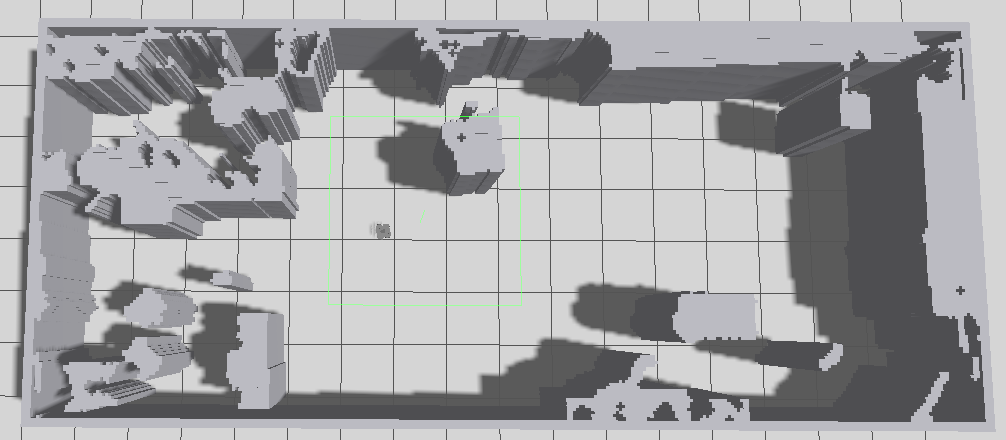
\includegraphics[width=0.85\textwidth]{figures/fig6_gazebo.png}
  \caption{The physics-based Gazebo simulation environment, built by extruding
  the 2D occupancy projection of a real survey-grade scan of the test room into
  a 3D world; the differential-drive platform explores it under the
  Cartographer/Nav2 stack.}
  \label{fig:gazebo}
\end{figure}

\begin{figure}[!htb]
\centering
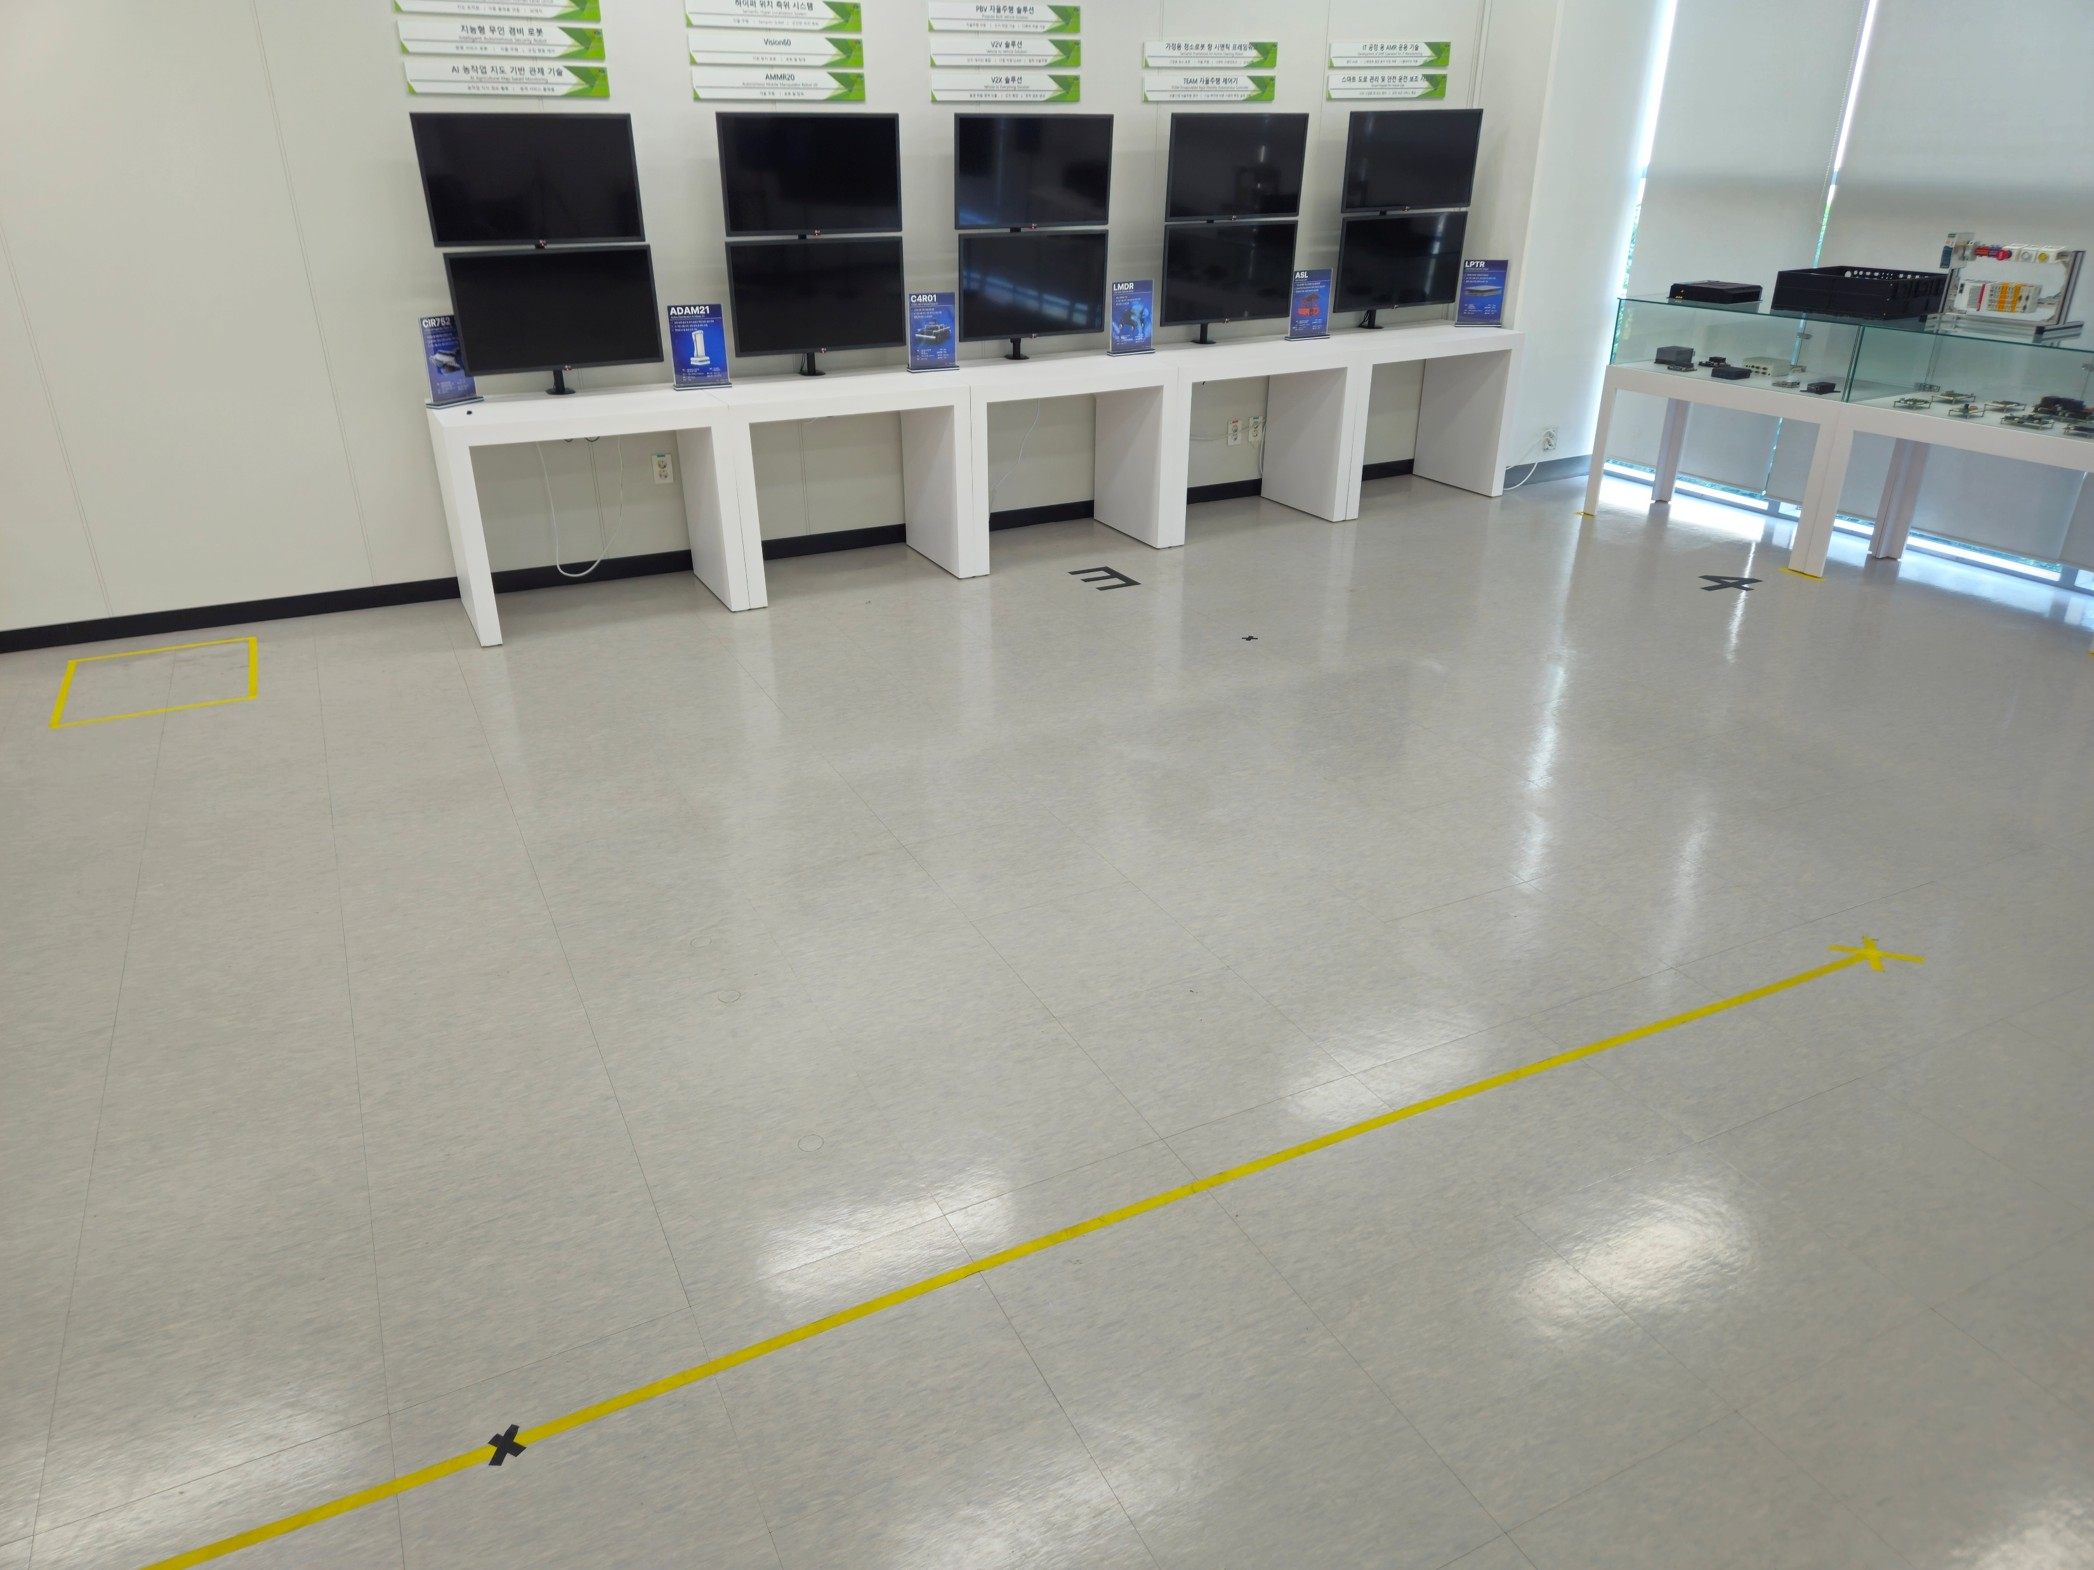
\includegraphics[width=0.9\linewidth]{figures/sen_fig10_testroom.jpg}
\caption{Physical industrial test room used for the hardware experiments and
for all semantic modeling scenes.}
\label{fig:testroom}
\end{figure}

For semantic modeling, the same room is observed across three scan epochs of
its working life, a property exploited deliberately (Table~\ref{tab:scenes},
Figure~\ref{fig:photos}). The \emph{showroom} epoch (T1, June 2026) captures
the room in an exhibition configuration, scanned manually with the door open.
The \emph{robot hall} epoch (T2, July 2026) captures the same room reorganized
as a robot test hall, scanned by autonomous visibility-driven exploration. A
third epoch (T3, late July 2026) adds a controlled-change re-scan at 99.6\%
LOS coverage. Because the two primary epochs differ in layout, furnishing, and
scan modality, they function as independent scenes for per-epoch evaluation
while enabling a real multi-epoch update study. A separate scene---a carpeted
\emph{cafeteria} with sofa booths and vending machines on the eighth floor of
the same building, scanned in August 2026 (57~M points, 28 clusters)---is held
out of the main campaign and used only as a cross-floor, out-of-vocabulary
stress case. Table~\ref{tab:sampleflow} connects every cluster set used in
this chapter to its derivation stage.

\begin{figure}[!htb]
\centering
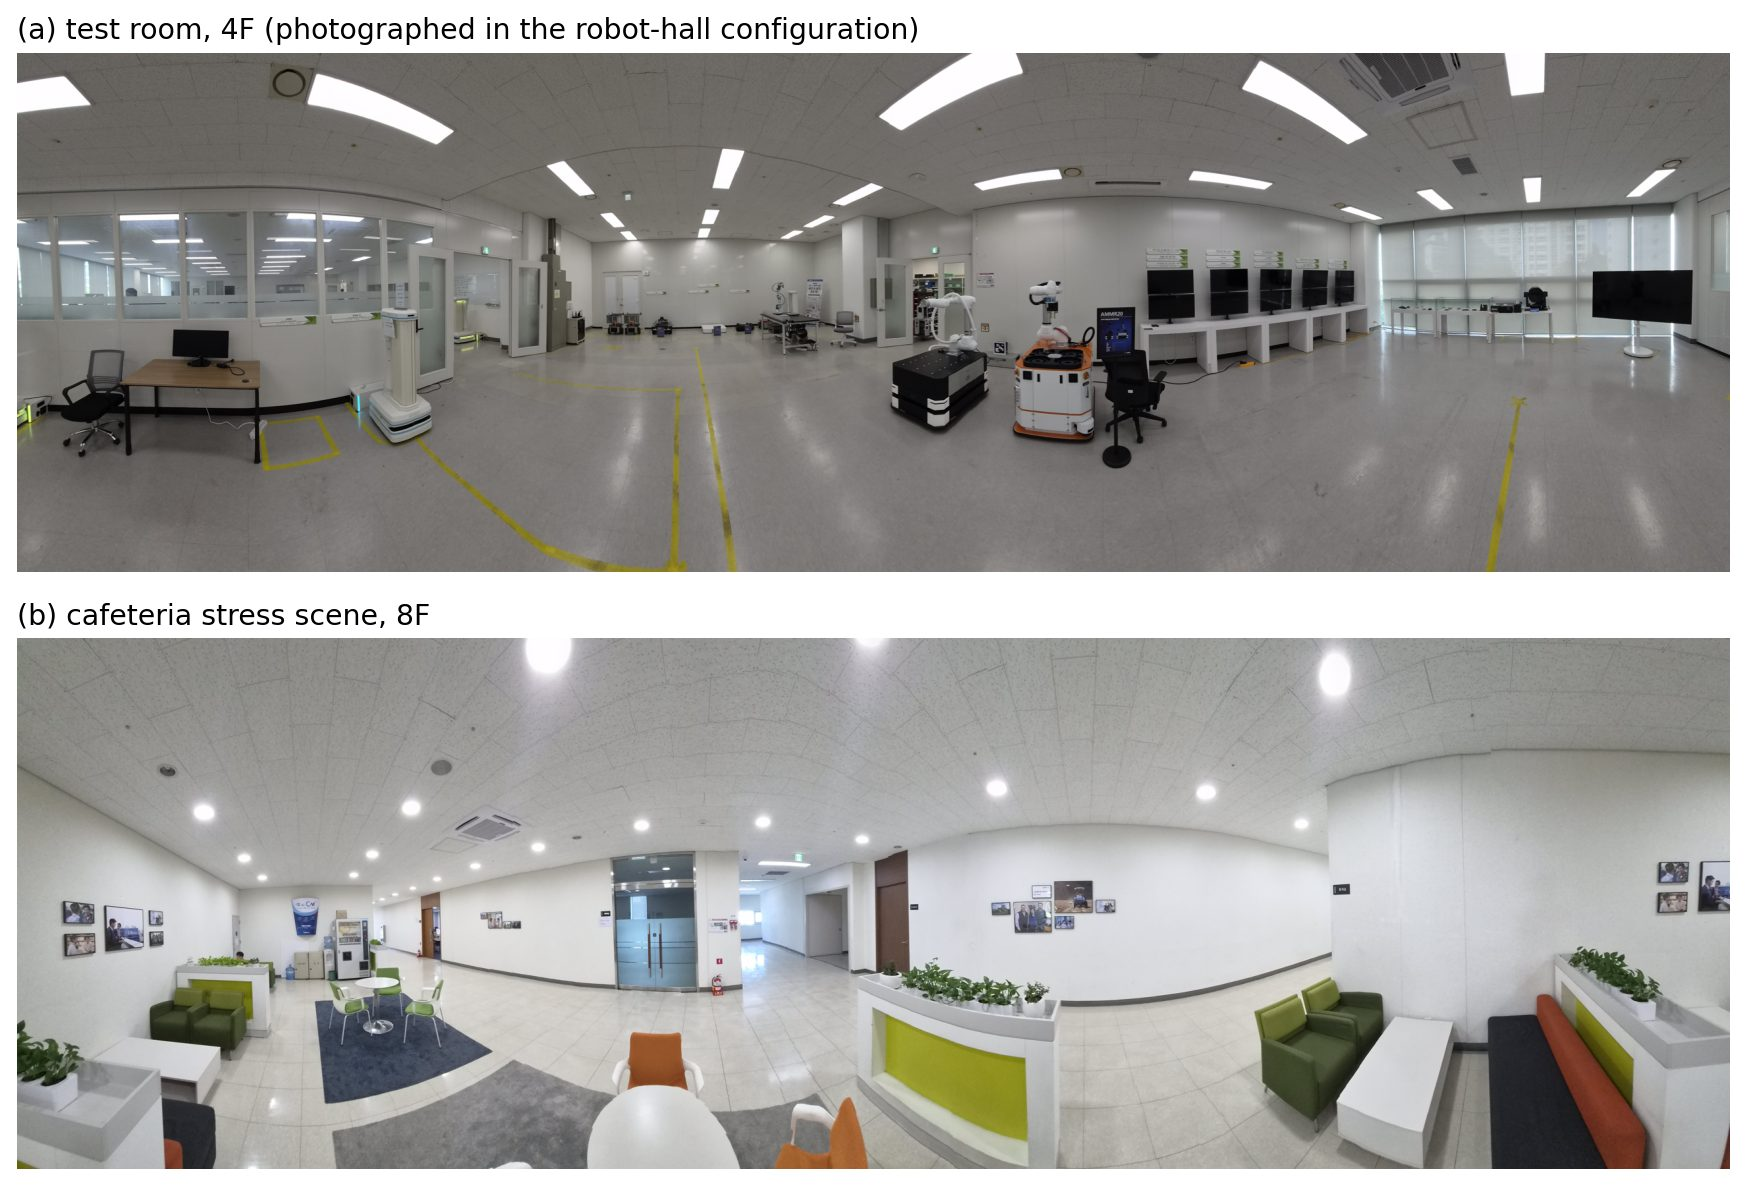
\includegraphics[width=\linewidth]{figures/ele_fig18_scene_photos.jpg}
\caption{The two semantic-modeling sites. (a)~The 4F test room in its
robot-hall configuration (T1 is an earlier furnishing of the same room;
visible: the AMMR platforms, the wall-mounted monitor bank, and a disinfection
robot). (b)~The 8F cafeteria stress scene: fabric sofas, planter partitions,
the vending row, and the brown door recovered by escalation on full-resolution
renders.}
\label{fig:photos}
\end{figure}

\begin{table}[htbp]
\centering
\caption{Scene statistics (deterministic detection sets after
structure-remnant filtering). T1 semantic processing starts from a manually
wall-removed export (4.9~M points) of the 46.3~M-point raw scan.}
\label{tab:scenes}
\small
\begin{tabularx}{\textwidth}{X c c c}
\toprule
 & \textbf{Showroom (T1)} & \textbf{Robot hall (T2)} & \textbf{Re-scan (T3)} \\
\midrule
Scan mode & manual, 1 setup & exploration & exploration, 6 setups \\
Raw points & 46.3M & 68.6M & 70.2M \\
Clean cloud (post-removal) & --- & 267K & 294K \\
Objects (filtered) & 38 & 81 & 79 \\
Room-scoped & 38 & 55 & 41 \\
Removed planes & 10 & 10 & 10 \\
\bottomrule
\end{tabularx}
\end{table}

\begin{table}[htbp]
\centering
\caption{Evaluation-set lineage: how every cluster set used in this chapter
derives from its scan ($\dagger$: grounded only in the experiment log;
``conf.''\,=\,ground-truth confirmed).}
\label{tab:sampleflow}
\small\setstretch{1.15}
\begin{tabularx}{\textwidth}{l X}
\toprule
\textbf{Lineage} & \textbf{Stage flow (cluster counts)} \\
\midrule
Showroom 57-set (Section~\ref{sec:exp-verify}) & 30 pre-split $\rightarrow$ 57 split $\rightarrow$ 50 after soffit filter $\rightarrow$ 50 GT-scored (36 conf.) \\
Showroom det set & 45 raw $\rightarrow$ 38 after soffit filter $\rightarrow$ 38 room-scoped \\
Robot hall det & 88 raw $\rightarrow$ 81 filtered $\rightarrow$ 55 room-scoped $\rightarrow$ 51 GT-scored (32 conf.) \\
T3 det1 & 79 merged $\rightarrow$ 41 room-scoped (= owner audit set) $\rightarrow$ 26 filter survivors \\
T3 det2 (precut) & 66 $\rightarrow$ 35 room-scoped $\rightarrow$ 27 to VLM (8 wall sheets excluded) \\
T3 det3/det4 & 33 consolidated $\rightarrow$ 46$^{\dagger}$ adjudicated \\
Cross-epoch KG (present) & rev7$\rightarrow$14: 47, 49, 51, 63, 64, 64, 46, \textbf{46} (current) \\
Frozen re-run (Section~\ref{sec:exp-endtoend}) & 66 $\rightarrow$ 35 in-room, scored vs.\ the 46-object graph \\
Cafeteria 8F & 28 $\rightarrow$ 25 GT-scored (20 conf.) \\
\bottomrule
\end{tabularx}
\end{table}

\subsection{Ground Truth and Annotation Protocol}
\label{subsec:gt}

Ground truth for semantic modeling was established in two passes: a
render-based audit of every cluster, followed by confirmation from the room's
owner (the facility operator) by physical inspection. Labels are graded
\emph{confirmed} (owner-verified), \emph{plausible}, or \emph{unknown};
accuracy is reported against confirmed ground truth (with lenient variants
including plausible where stated), unknown objects are excluded, and structure
artifacts are tracked separately. The showroom verification study uses the
original 57-cluster decomposition, of which 50 are scored after excluding 7
structure artifacts (confirmed 36 / plausible 12 / unknown 2); the room-scoped
robot hall has 51 scored clusters (confirmed 32); the cafeteria has 25 of 28
(confirmed 20). Both audit passes share an anchoring channel---the render
audit presents proposed labels that the owner then corrects---so confirmed
grades are owner decisions over physically known rooms rather than blind
annotations. To measure this bias directly, two blind annotations were added.
A co-author familiar with the facility who had seen neither the T3 pipeline
output nor the owner audit labeled all 41 T3 clusters blind from
full-resolution multi-view render sheets carrying only shuffled identifiers:
on the 33 clusters both annotators labeled, the blind labels agree with the
owner's on 31 (93.9\%), and on the clusters where the owner had overturned the
pipeline label the blind annotator independently reproduced the override on 25
of the 26 scored. An external annotator with no connection to the work and
no familiarity with the facility labeled the same 41 sheets under the same
protocol: without site knowledge, agreement with the owner drops to 21 of 33
(63.6\%), but 16 of 19 labels given at confidence 4--5 agree (84\%), and 11 of
the 12 disagreements fall on absorbed or merged industrial objects and on
ceiling or wall remnants---the categories that required on-site knowledge in
the owner audit. The owner ground truth is therefore described as
anchoring-bounded rather than anchoring-free. For the mapping subsystem, a
ground-truth occupancy map of the simulated test room is maintained for
map-quality registration, and tape measurements provide the reference for the
twin's geometric fidelity.

\subsection{Metrics}
\label{subsec:metrics}

Table~\ref{tab:metrics} aligns the metrics with the five research objectives
of Section~\ref{sec:objectives}. For mapping (O1), the figure of merit is LOS
coverage (Equation~\ref{eq:los}); because each autonomous run maps a slightly
different extent of free space, every cross-run comparison re-evaluates all
runs on a single common reference map (the most complete map among the runs
compared) so that all runs share the same free-space denominator, and the scan
count is reported alongside as the cost term. Registration quality is measured
by the number of setups and links, the overall overlap, and the bundle error
reported by the registration software. For the backbone (O2), repeatability is hash-verified
byte identity of clusters, and instance quality is recall against an
owner-audited inventory in a membership-independent form. For verification
(O3), classification accuracy is top-1 against confirmed ground truth under
documented synonym-tolerant matching, and verification quality is per-tier
precision, recall, and $F_1$. For querying, a \emph{hallucination} is an
unsupported atomic factual claim, and the hallucination rate is the fraction
of unsupported claims over all factual claims. Update quality uses matching accuracy, identity-switch rate,
false-new and false-absent counts, and unchanged stability. For the twin and
missions (O4, O5), conversion time, simulation throughput, tape-measured scene
dimensions and checkpoint distances, and mission success, completion time, and
arrival error are reported.

\begin{table}[htbp]
  \centering
  \caption{Evaluation metrics aligned with the five research objectives.}
  \label{tab:metrics}
  \begin{tabularx}{\textwidth}{l X X}
    \toprule
    \textbf{Objective} & \textbf{Metric} & \textbf{Section} \\
    \midrule
    O1 & LOS coverage vs.\ scan count; registration setups/links/overlap/bundle error & \ref{sec:exp-mapping} \\
    O2 & Byte-identical repeatability; instance recall vs.\ owner inventory; proxy comparison vs.\ learned baselines & \ref{sec:exp-seg} \\
    O3 & Verification accuracy, per-tier precision/recall/$F_1$; query accuracy, hallucination rate, traps blocked; matching accuracy, identity switches; automated recall & \ref{sec:exp-verify}--\ref{sec:exp-ablation} \\
    O4 & Conversion time, scene complexity, simulation throughput, dimensional error, twin positioning error & \ref{sec:exp-twin} \\
    O5 & Mission success, completion time, arrival error, phantom-goal refusal & \ref{sec:exp-missions} \\
    \bottomrule
  \end{tabularx}
\end{table}

\paragraph{Controls and generative-AI use.}
The verifier for the main semantic campaign is fixed to a single model
(Claude Sonnet~4.6~\cite{anthropic2026}); every verification, escalation, and
owner interaction in the accumulated knowledge-graph lineage was produced under
this one verifier, so results remain comparable across sections. All query
conditions share the same LLM, system prompt, query set, decoding parameters,
and forced answer schema and differ only in the knowledge view they receive.
Constants in the base pipeline were fixed on T1/T2 and applied unchanged to T3
and the cafeteria; the corrective-layer thresholds were developed on the
test-room lineage and frozen before evaluation on the cafeteria. Generative
models enter this work in two strictly separated roles: as experimental
components under test (Stage-B verification, query answering, place naming,
and the five-verifier comparison), every call made under a forced schema with
prompts and usage archived; and as a writing aid for language editing of the
underlying manuscripts, with no role in study design, data collection, or
analysis.

\section{Automated Mapping Subsystem}
\label{sec:exp-mapping}

\subsection{Scan-Trigger Strategies in the Simulated Test Room}
\label{subsec:prelim-mapping}

The first experiment, carried over from the preliminary defense, establishes
why the scan/skip decision needs a coverage model at all. Two strategies are
contrasted in the simulated test room: a \emph{distance-traveled} trigger,
which fires a stationary survey scan whenever the platform has driven a fixed
path distance with no redundancy check, and the \emph{prior-scan-radius}
strategy of Section~\ref{subsec:proximity-rule}, which proposes a candidate at
the same interval but skips any candidate within straight-line distance $R$ of
an existing scan. Five configurations are compared (Table~\ref{tab:ablation0}):
the distance-traveled baseline, three settings sweeping $R$ from 3 to 5~m, and
one with frontier suppression disabled. The distance-traveled baseline stops
21 times to map the room; the prior-scan-radius strategy maps the same room
with three scans---a roughly seven-fold reduction in expensive stationary
acquisitions---by skipping the 21 to 27 candidates that fall within $R$ of an
existing scan. Sweeping $R$ trades scan count and travel time against room
coverage, and $R=4$~m, set with reference to the scanner's effective range, was
selected. Across every configuration the free-space IoU of the resulting
Cartographer map stays between 0.94 and 0.97 with a wall RMSE near 0.31~m:
because the 2D map is built continuously from the navigation laser while the
stationary survey scans serve the dense 3D capture, reducing the number of
stops does not degrade the navigation map (Figures~\ref{fig:mapscan}
and~\ref{fig:mapqual}). Disabling frontier suppression lowers the IoU slightly
because abandoned frontiers are reapproached and inject minor drift. The
sequencer also behaves correctly under the survey-scanner timing model:
in-place rotation does not trigger scans, the capture--download decoupling lets
the platform resume motion during background downloads without overlapping
acquisitions, and the reconnect path recovers from simulated connection losses
up to the configured retry bound.

\begin{table}[htbp]
  \centering
  \caption{Scan-triggering strategies in the simulated test room
  (ground-truth free area 85.5~m$^2$; room coverage = fraction of free area
  within straight-line distance $R$ of some scan; overlap =
  $1-A_{\mathrm{cov}}/A_{\mathrm{sum}}$ over disks of radius $R$). Source:
  ICCAS~2026~\cite{iccas2026}.}
  \label{tab:ablation0}
  \footnotesize\setstretch{1.15}
  \begin{tabularx}{\textwidth}{X c c r r r r r r}
    \toprule
    \textbf{Strategy} & $R$ (m) & Supp. & Scans & Skip. & Time (s) & Overlap & Room (\%) & IoU$_{\mathrm{free}}$ \\
    \midrule
    distance-traveled   & ---  & yes & \textbf{21} & 0  & 692 & ---   & ---   & 0.965 \\
    prior-scan $R3$   & 3.0  & yes & 5  & 21 & 416 & 0.241 & 88.2  & ---   \\
    prior-scan $R4$ (selected) & 4.0 & yes & \textbf{3} & 27 & 357 & 0.164 & 91.0 & \textbf{0.965} \\
    prior-scan $R5$   & 5.0  & yes & 3  & 22 & 309 & 0.222 & \textbf{98.9}  & 0.956 \\
    prior-scan $R4$, no supp. & 4.0 & no & 3 & 24 & 339 & 0.166 & 93.6 & 0.938 \\
    \bottomrule
  \end{tabularx}
\end{table}

\begin{figure}[!htb]
  \centering
  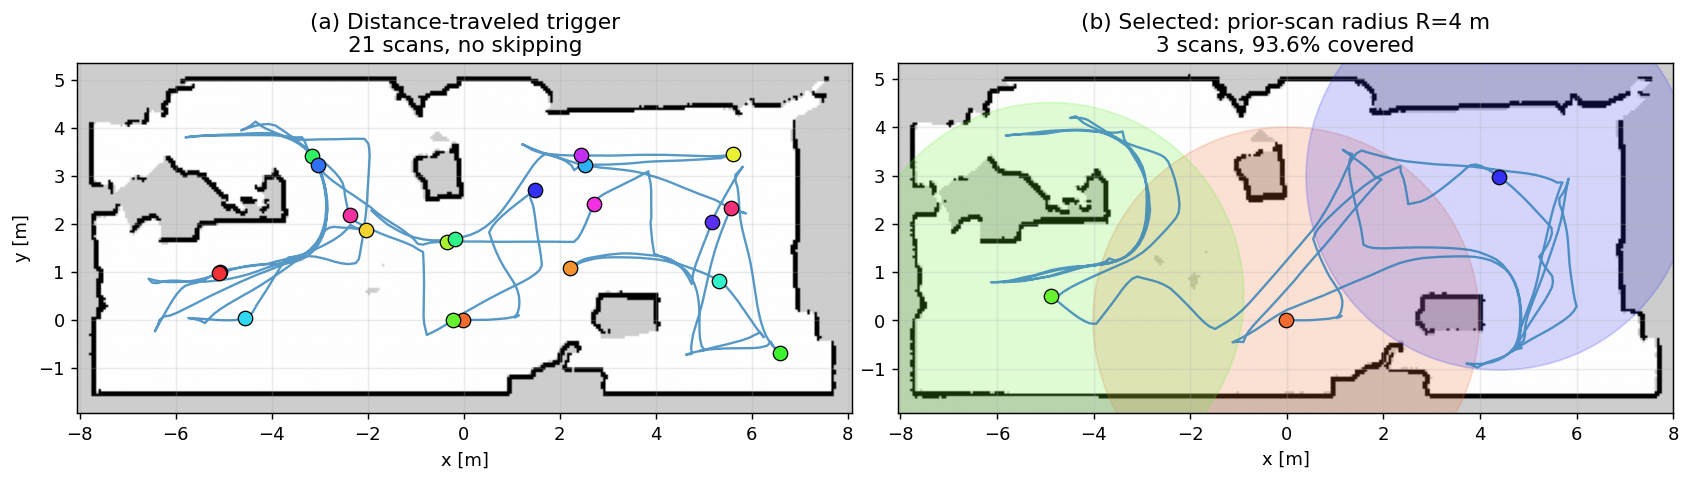
\includegraphics[width=\textwidth]{figures/fig6_strategy.png}
  \caption{Scan-triggering strategies overlaid on the Cartographer SLAM map
  (shaded disks: the skip radius $R$ around each scan; solid line: the robot
  trajectory; markers: scan positions). (a)~The distance-traveled trigger
  fires 21 scans. (b)~The prior-scan radius ($R=4$~m) maps the room with 3
  scans.}
  \label{fig:mapscan}
\end{figure}

\begin{figure}[!htb]
  \centering
  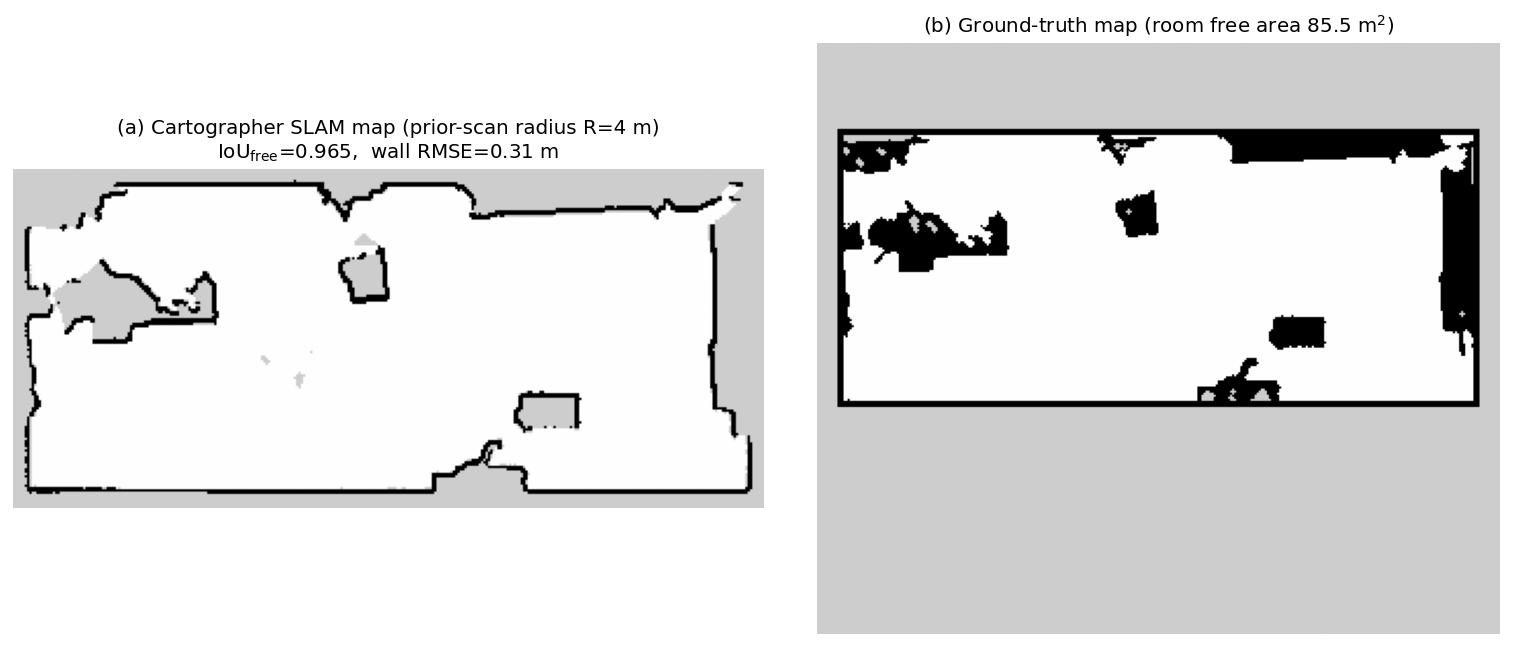
\includegraphics[width=0.92\textwidth]{figures/fig6_mapqual.png}
  \caption{Map quality of the selected run ($R=4$~m). (a)~The Cartographer
  occupancy map, $\mathrm{IoU}_{\mathrm{free}}=0.965$ and wall RMSE 0.31~m
  after translation alignment to ground truth. (b)~The ground-truth occupancy
  map of the test room.}
  \label{fig:mapqual}
\end{figure}

The proximity rule, however, judges coverage by Euclidean distance alone. The
remainder of this section evaluates the visibility-based policy of
Sections~\ref{sec:coverage} and~\ref{sec:placement} on two axes, LOS coverage
and stationary scan count. Four placement policies are compared throughout:
(i)~a \emph{uniform no-skip} reference that scans at every candidate---an
upper reference on the coverage attainable along a path; (ii)~the \emph{disk
spacing} baseline above; (iii)~the \emph{disk marginal-gain} baseline, which
applies the identical accept/skip rule as the proposed policy to the disk
coverage model; and (iv)~the proposed \emph{ray-cast visibility} policy.
Published TLS scan-planning methods are not applicable as online baselines
because they optimize viewpoints offline over a prior environment
model~\cite{tls-scanplanning,dehbi2021,knechtel2025}.

\subsection{Coverage Model and Single-Room Placement}
\label{subsec:exp-singleroom}

Figure~\ref{fig:concept} contrasted the two coverage models for a single scan
pose. On the full single-room world, the visibility stop-and-scan policy
places four scans and reaches 97.9\% LOS coverage
(Figure~\ref{fig:singleroom}). Varying the range bound $R\in\{5,6,10\}$~m
yields 97--98\% LOS in all cases (Figure~\ref{fig:rsweep}); larger $R$ needs
fewer scans but spreads them apart, reducing inter-scan overlap. $R=6$~m is
adopted for three reasons: it balances coverage against the scan-to-scan
overlap that registration benefits from; it keeps every cell claimed as
covered well inside the scanner's highest-accuracy band (3D point accuracy of
6~mm at 10~m~\cite{leica-blk360}); and it matches the local room scale, and
hence the occlusion scale, of the indoor environments targeted.

\begin{figure}[!htb]
\centering
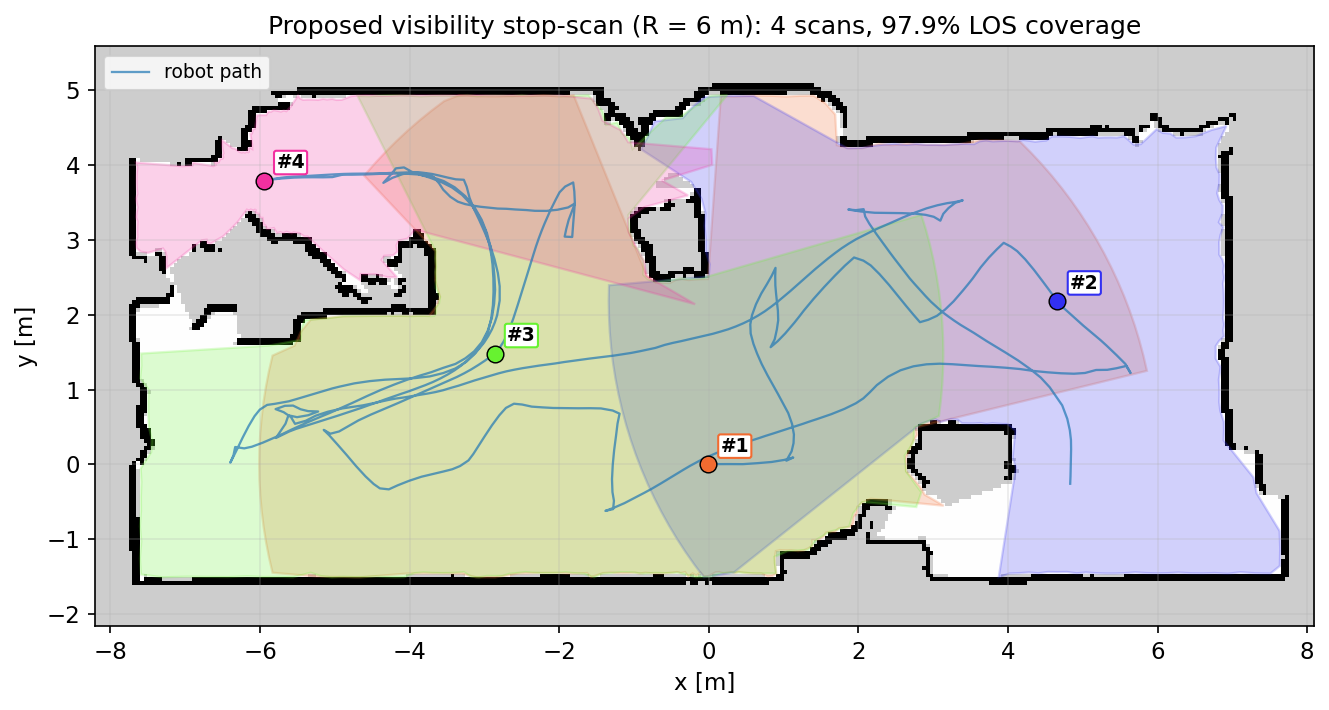
\includegraphics[width=0.7\linewidth]{figures/sen_fig2_singleroom_sota.png}
\caption{Visibility stop-and-scan on the single-room world ($R=6$~m): 4~scans,
97.9\% LOS coverage. Each accepted scan pose (marker) and its visibility
polygon share one color, indexed by scan order; the grayscale background is
the occupancy map and the blue line the robot path.}
\label{fig:singleroom}
\end{figure}

\begin{figure}[!htb]
\centering
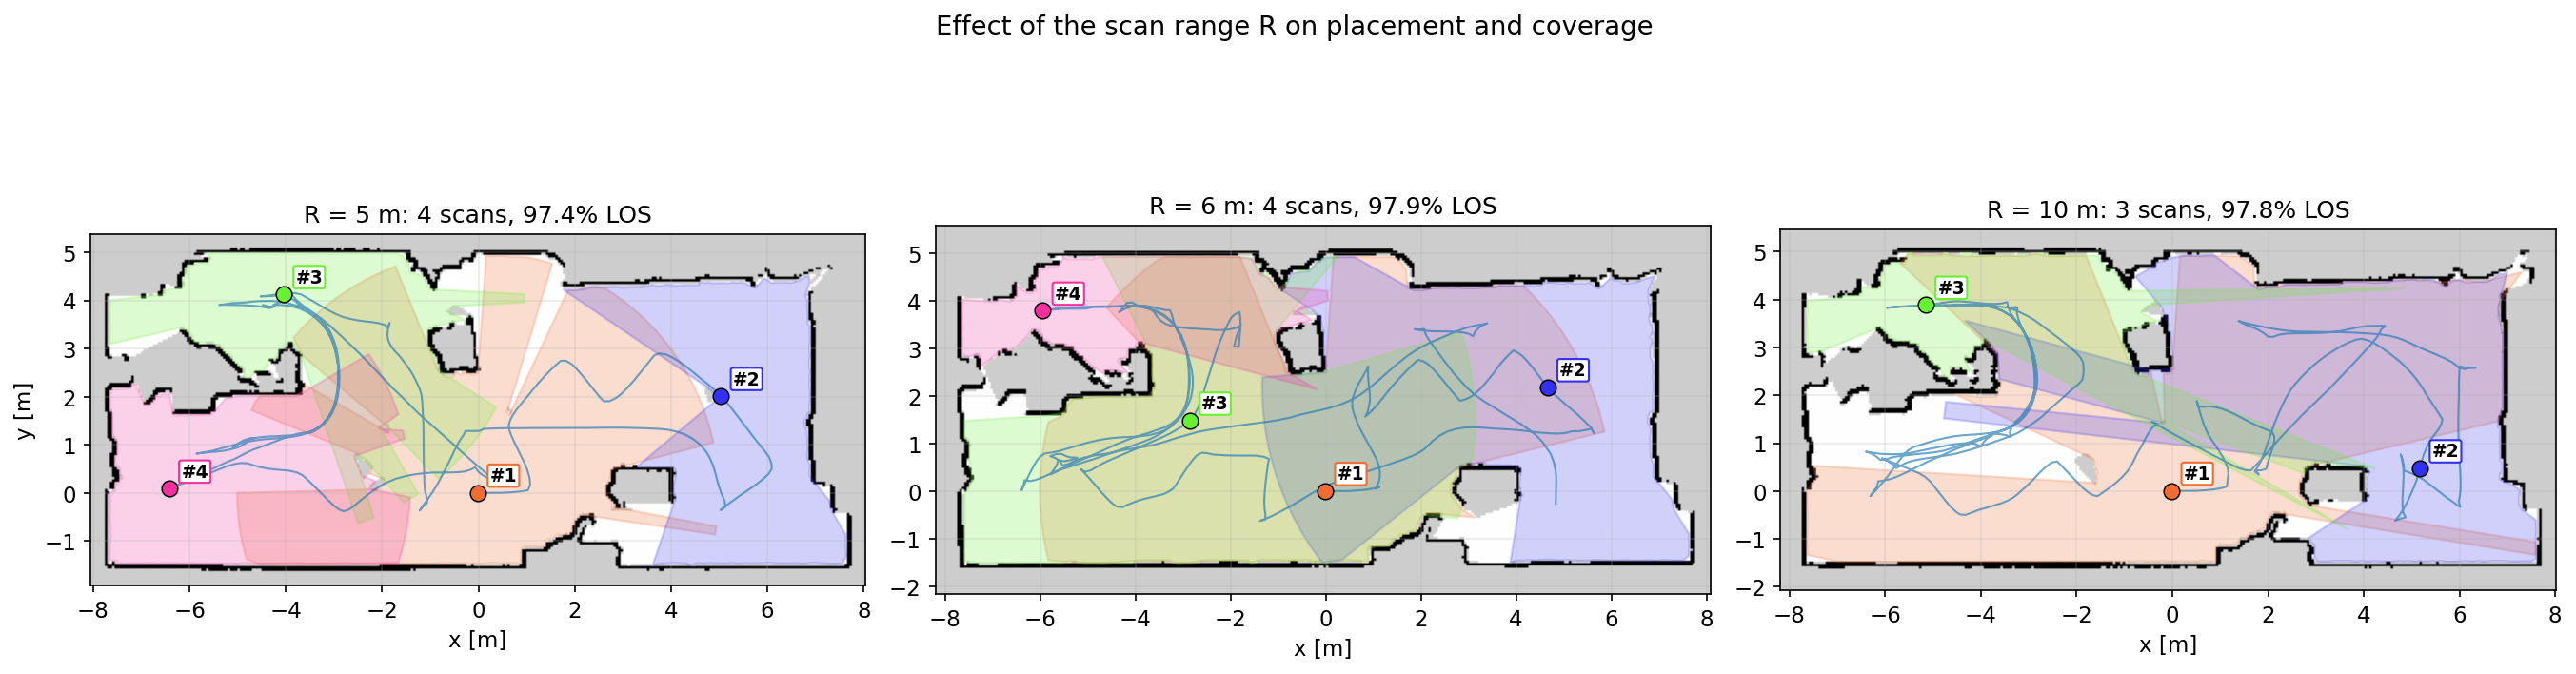
\includegraphics[width=0.95\linewidth]{figures/sen_fig3_R_sweep.png}
\caption{Effect of the range bound $R$ on placement and coverage for
$R=5/6/10$~m. Larger $R$ needs fewer scans but spreads them; $R=6$~m balances
coverage (97.9\%) against inter-scan overlap for registration.}
\label{fig:rsweep}
\end{figure}

\subsection{Controlled Skip-Rule Ablation}
\label{subsec:exp-ablation}

The decisive comparison isolates the only variable of interest, the
accept/skip decision, from the stochasticity of autonomous exploration. On a
fixed environment map and a fixed candidate sequence (a logged trajectory
resampled every 2~m of path length, denser than the live 3~m trigger so that no
policy is starved of decision opportunities), \emph{all} policies are
replayed, so they see identical maps and identical candidate poses and differ
only in which candidates they accept (Figure~\ref{fig:ablation}). This
deterministic, paired design removes the confound that, in live runs, which
rooms get mapped is dominated by navigation through narrow doorways rather
than by the skip rule.

Across $N=5$ single-room and $N=10$ multi-room trajectories, the visibility
rule raises LOS coverage from $77.0\pm4.9\%$ to $85.4\pm6.2\%$ in the
single-room world and from $77.0\pm6.4\%$ to $84.0\pm9.2\%$ in the three-room
world, at a cost of one to two additional scans on average
(Table~\ref{tab:ablation}, Figure~\ref{fig:summary}). The uniform no-skip
reference reaches $91.9\pm7.0\%$ and $86.6\pm9.9\%$ LOS, but at 28.0 and 40.8
scans on average; the visibility rule comes within 6.5 and 2.6 percentage
points of this brute-force upper reference while taking roughly an eighth as
many scans, and exceeds the disk baseline by $+8.4$ and $+7.0$ points. On
paths that traverse every room, where the disk rule's blindness to occlusion
is fully exercised, the per-path gain reaches $+21$ to $+23$ points. The disk
spacing rule is structurally capped: once two scans are placed, almost every
later candidate lies within $R$ of a prior scan, so it stops scanning even
though walls occlude much of the area it counts as covered.

The disk marginal-gain baseline isolates the coverage model from the
acceptance rule. Under the identical dual criterion, the disk model accepts
$2.6\pm0.5$ scans for $77.7\pm3.8\%$ LOS in the single-room world---essentially
the spacing rule's result---and $2.9\pm0.3$ scans for only $59.1\pm1.3\%$ LOS
in the multi-room world, markedly \emph{worse} than even the spacing rule.
Because $B_{\mathrm{disk}}$ claims area through partitions, the disk model's
own coverage bookkeeping saturates after the first few acceptances: every
later candidate appears almost fully covered, so the rule stops scanning while
whole rooms remain unobserved. That the same acceptance rule produces a
24.9-point LOS gap between the two coverage models in the multi-room world is
the sharpest form of this dissertation's claim: the deficiency lies in the
disk coverage model itself, not in the acceptance rule attached to it.

\begin{table}[htbp]
\centering
\caption{Controlled skip-rule ablation: four placement policies replayed on
the same fixed candidate sequences ($N=5$ single-room, $N=10$ multi-room
paths); mean\,$\pm$\,s.d. All policies traverse the identical path, so they
differ only in scan count. Source: \emph{Sensors}~\cite{kim2026sensors}.}
\label{tab:ablation}
\begin{tabular}{l l c c}
\toprule
\textbf{Environment} & \textbf{Coverage model} & \textbf{LOS coverage (\%)} & \textbf{Scans} \\
\midrule
\multirow{4}{*}{Single-room} & Uniform, no skip (reference) & $91.9\pm7.0$ & $28.0\pm13.0$ \\
                             & Disk, spacing rule (baseline) & $77.0\pm4.9$ & $2.0\pm0.0$ \\
                             & Disk, marginal-gain rule      & $77.7\pm3.8$ & $2.6\pm0.5$ \\
                             & Ray-cast visibility (ours)   & $\mathbf{85.4\pm6.2}$ & $3.6\pm0.9$ \\
\midrule
\multirow{4}{*}{Multi-room}  & Uniform, no skip (reference) & $86.6\pm9.9$ & $40.8\pm11.8$ \\
                             & Disk, spacing rule (baseline) & $77.0\pm6.4$ & $2.3\pm0.5$ \\
                             & Disk, marginal-gain rule      & $59.1\pm1.3$ & $2.9\pm0.3$ \\
                             & Ray-cast visibility (ours)   & $\mathbf{84.0\pm9.2}$ & $3.6\pm0.7$ \\
\bottomrule
\end{tabular}
\end{table}

\begin{figure}[!htb]
\centering
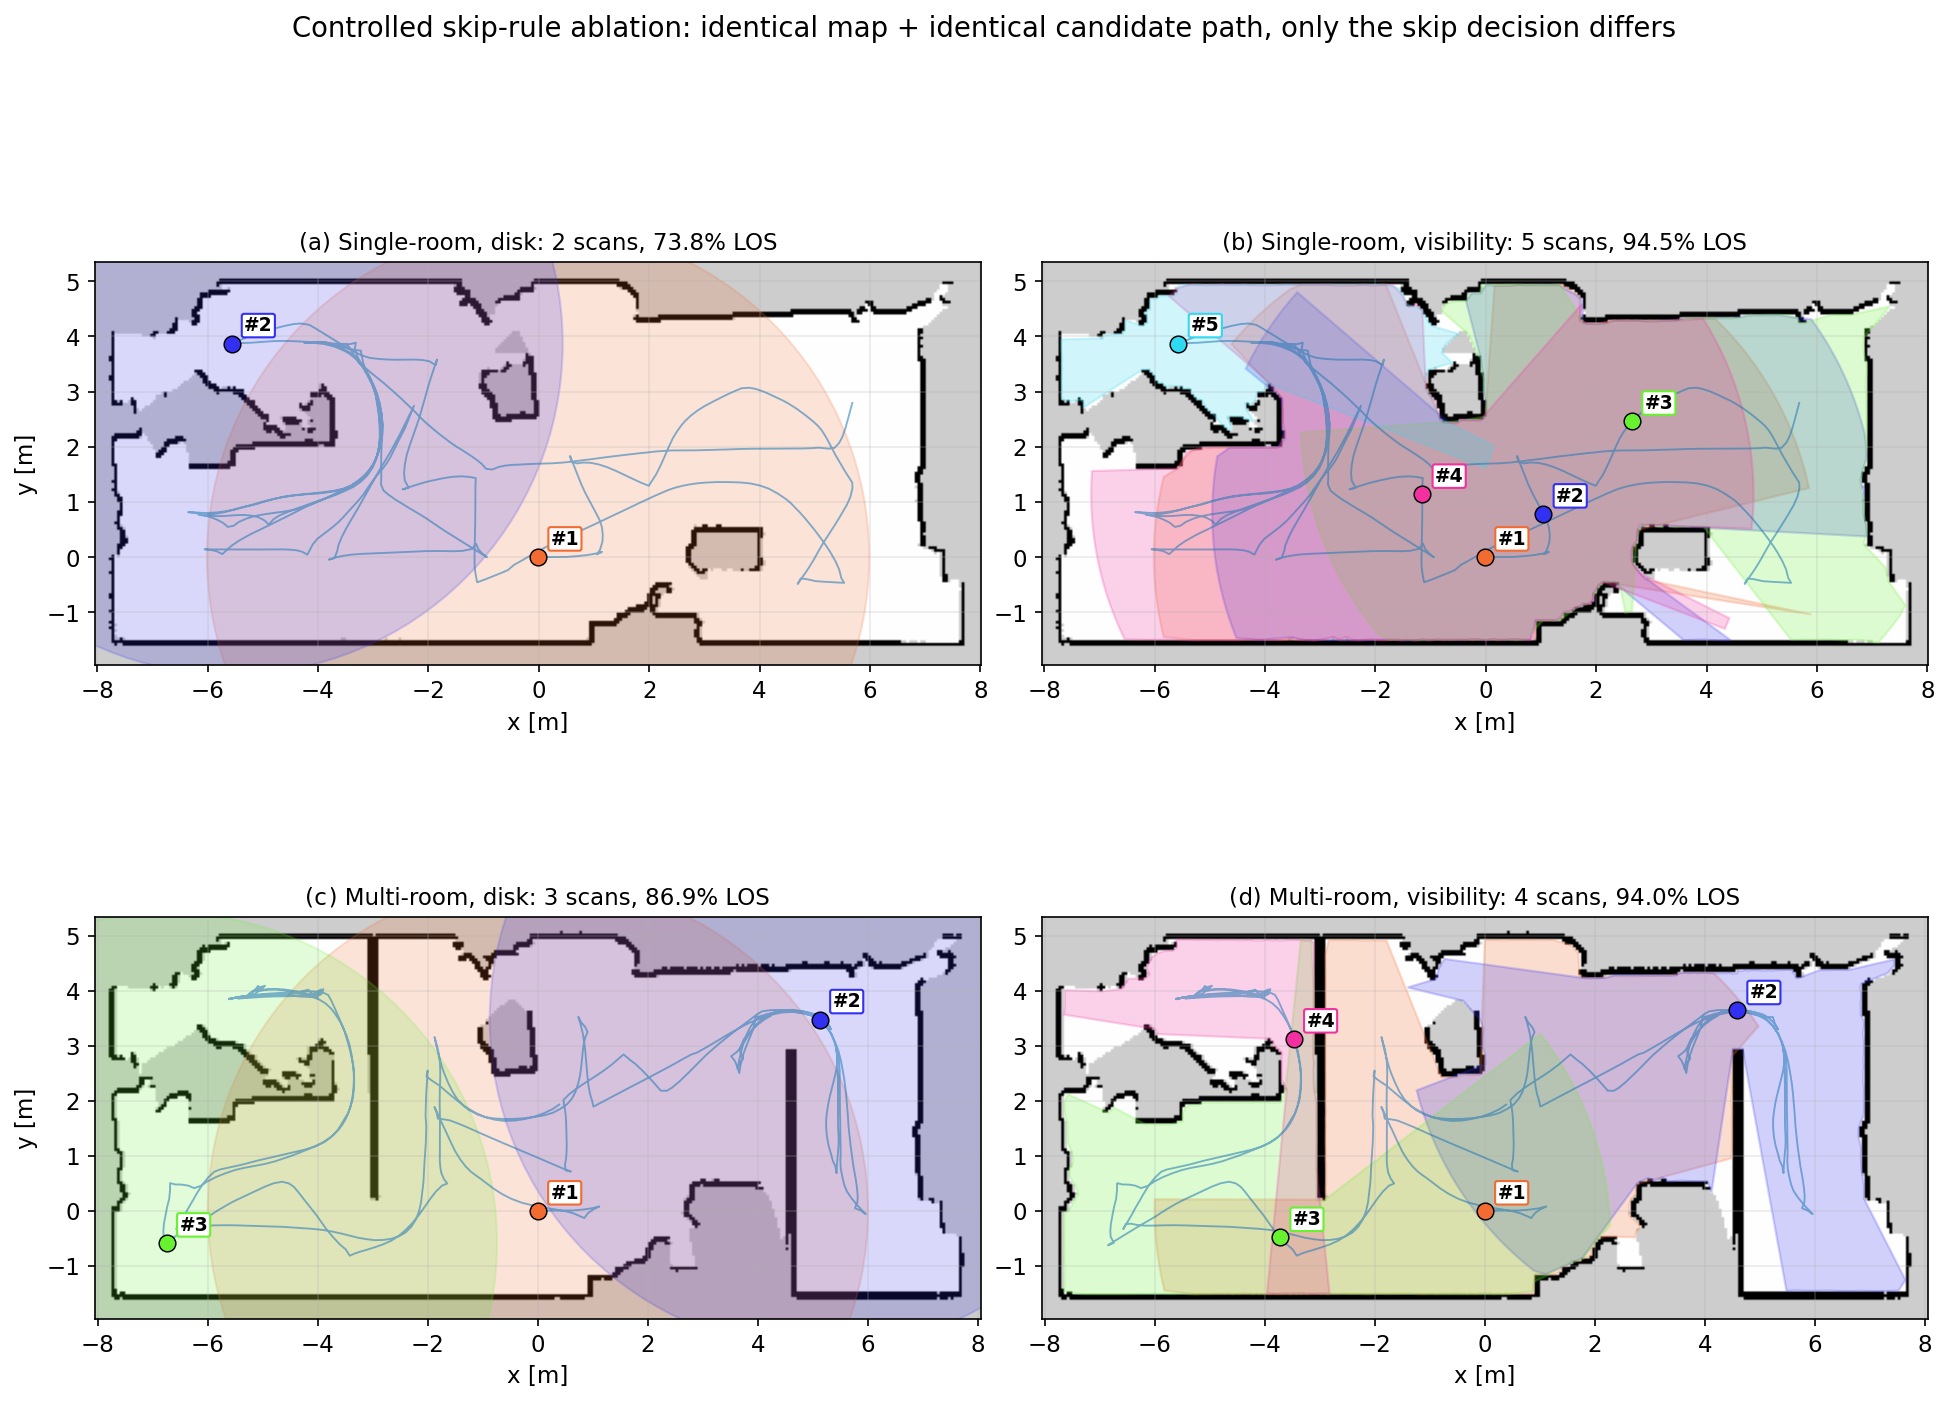
\includegraphics[width=0.95\linewidth]{figures/sen_fig5_skip_ablation.png}
\caption{Controlled skip-rule ablation on an identical map and candidate
path; only the skip decision differs. (a,b)~Single-room and (c,d)~multi-room,
under the disk spacing rule (a,c) and the visibility rule (b,d).}
\label{fig:ablation}
\end{figure}

\begin{figure}[!htb]
\centering
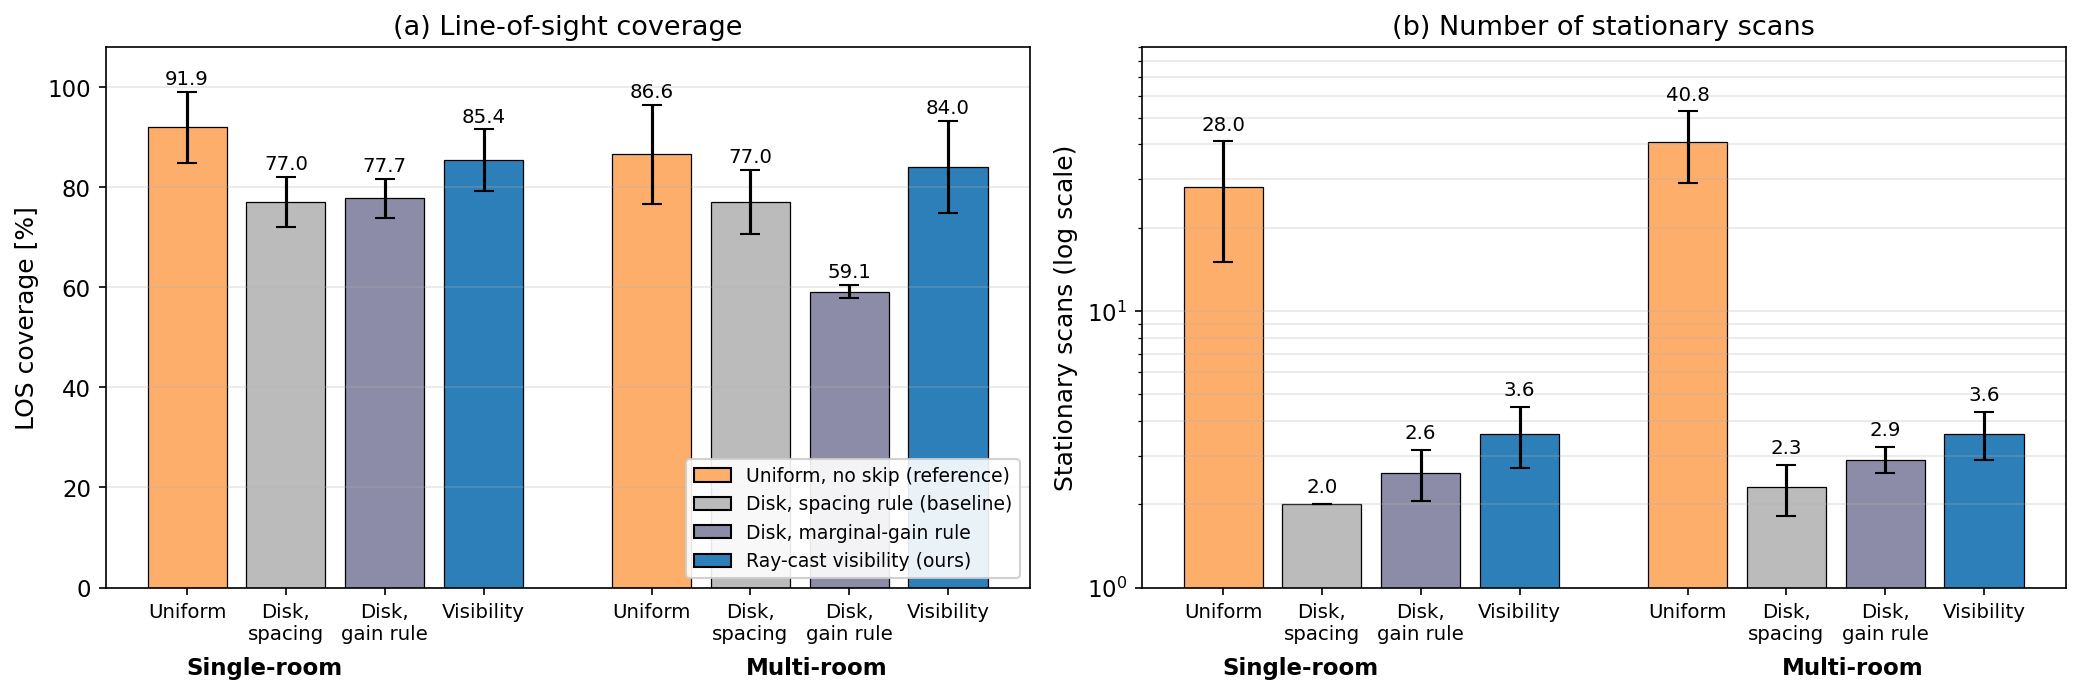
\includegraphics[width=0.95\linewidth]{figures/sen_fig7_summary.png}
\caption{Four-way skip-rule comparison on identical paths ($N=5$ single-room,
$N=10$ multi-room trajectories, paired per path). (a)~LOS coverage;
(b)~stationary scan count, log scale (mean\,$\pm$\,s.d.).}
\label{fig:summary}
\end{figure}

\subsection{Live Multi-Room Demonstration, Coverage Completion, and Parameter Sensitivity}
\label{subsec:exp-sensitivity}

Figure~\ref{fig:multiroom} shows a single live autonomous run on the
multi-room world under each coverage model. The disk policy stops after two
scans at 46.9\% LOS, having counted an entire room behind a partition as
covered through the wall; the visibility policy places one scan per room,
three in total, and reaches 95.1\% LOS. This run is presented as a qualitative
demonstration: in live runs on the partitioned world, which rooms get mapped
varies from run to run and dominates the measured coverage largely
independently of the skip rule, so the rigorous claim is the controlled
ablation above. With the coverage-completion phase enabled, the robot continues
after frontier convergence to drive into and scan the remaining uncovered
pockets: over $N=5$ runs this raises LOS coverage to $98.9\pm0.9\%$ using
$5.0\pm1.2$ total scans on average (3.2 frontier plus 1.8 completion scans),
with no unreachable pockets; a representative run reaches 99.6\% LOS
(Figure~\ref{fig:completion}).

\begin{figure}[!htb]
\centering
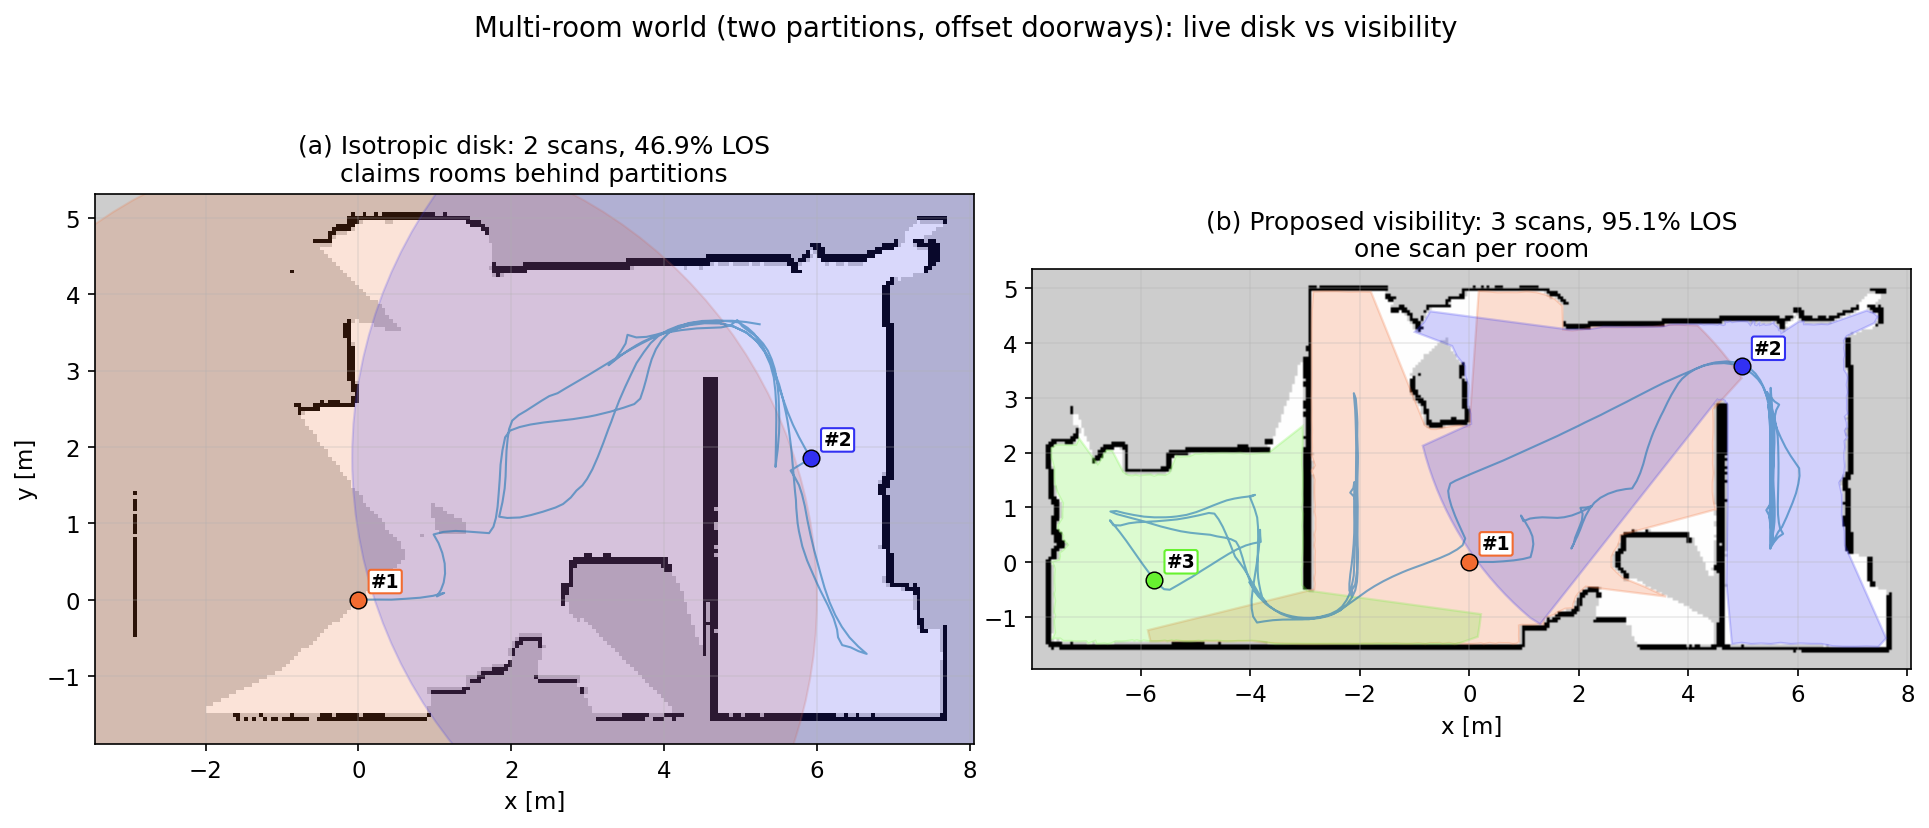
\includegraphics[width=0.95\linewidth]{figures/sen_fig4_multiroom_compare.png}
\caption{Multi-room world (two partitions, offset doorways): live disk vs.\
visibility. (a)~The disk model skips candidates within $R$ of a prior scan
through the partitions, giving 2~scans and 46.9\% LOS with a whole room
unscanned. (b)~The visibility model scans once per room, giving 3~scans and
95.1\% LOS.}
\label{fig:multiroom}
\end{figure}

\begin{figure}[!htb]
\centering
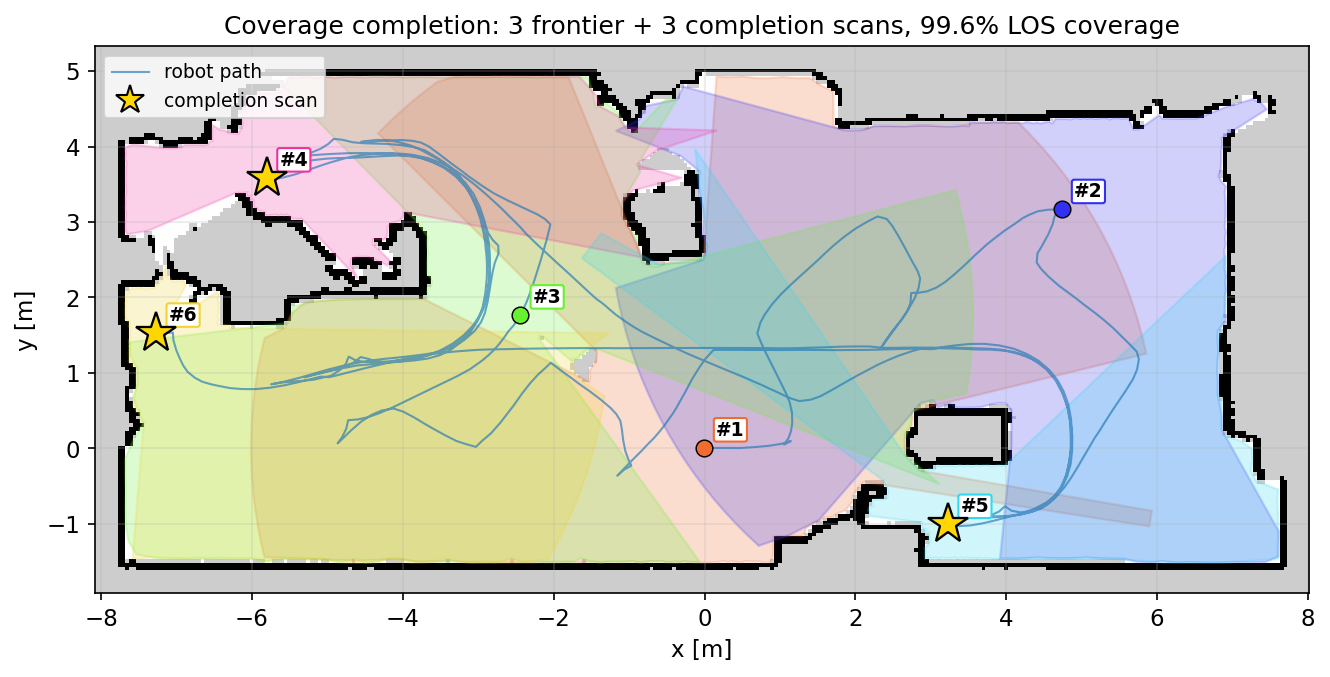
\includegraphics[width=0.7\linewidth]{figures/sen_fig6_completion.png}
\caption{Coverage completion. After frontier exploration, the robot drives
into each still-uncovered pocket and scans ($\star$) until none above the
minimum pocket area remains. Here 3~frontier $+$ 3~completion scans, 99.6\%
LOS.}
\label{fig:completion}
\end{figure}

The two skip thresholds are characterized by deterministic replay of the
visibility policy over the same fixed paths (Figure~\ref{fig:sweep}). Varying
the relative threshold $\tau$ over $[0.10,0.50]$ changes mean LOS coverage by
at most about two points (single-room $86.4\to84.3\%$; multi-room
$85.2\to84.0\%$) and mean scan count by less than one scan, so $\tau=0.30$ is
not a sensitive choice. The absolute threshold $A_{\min}$ is the operative
knob: $A_{\min}=5$~m$^2$ is the largest threshold whose mean LOS remains within
about five points of the most aggressive setting ($A_{\min}=1$~m$^2$) in both
environments (single-room 85.4 versus 90.7\%; multi-room 84.0 versus 85.7\%)
while already halving the scan count (3.6 versus 7.2 scans). Beyond the knee
the trade turns unfavorable: $A_{\min}=15$~m$^2$ saves only about one further
scan while coverage continues to erode ($85.4\to80.8\%$ and
$84.0\to83.1\%$). The operating point $\tau=0.30$, $A_{\min}=5$~m$^2$ was
fixed before the hardware campaign.

\begin{figure}[!htb]
\centering
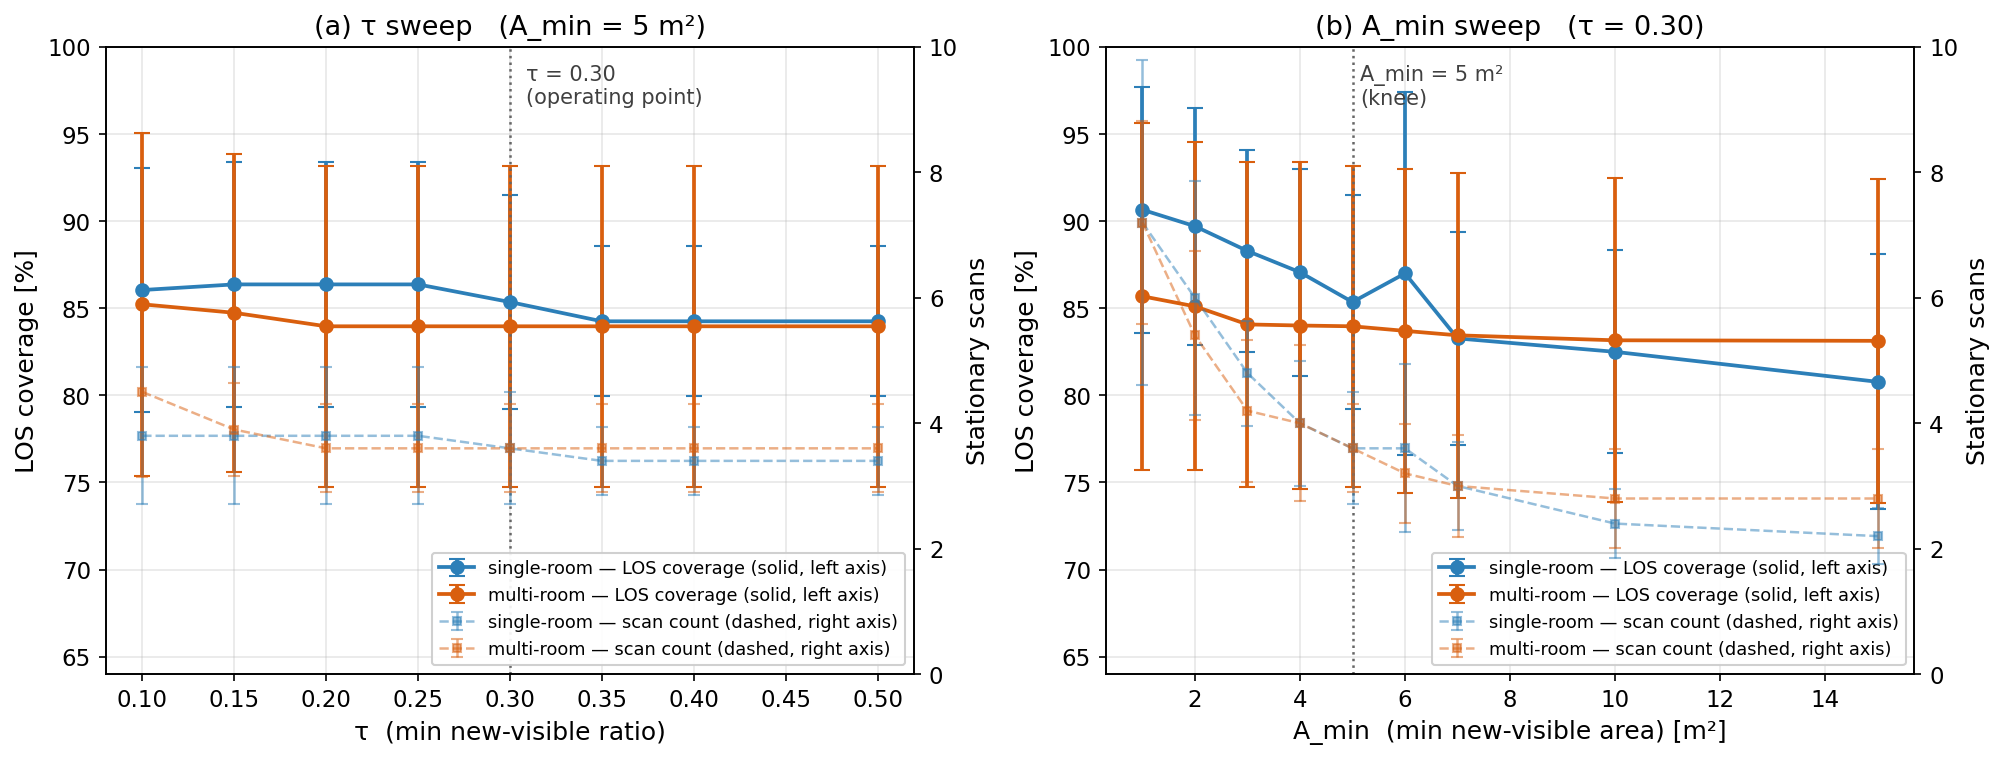
\includegraphics[width=0.95\linewidth]{figures/sen_fig8_param_sweep.png}
\caption{Parameter sweep by deterministic replay on the fixed candidate paths
(mean~$\pm$~s.d.). Solid curves: LOS coverage; dashed curves: scan count.
(a)~$\tau$ sweep at $A_{\min}=5$~m$^2$; (b)~$A_{\min}$ sweep at $\tau=0.30$,
knee marked.}
\label{fig:sweep}
\end{figure}

\subsection{Fully Autonomous On-Hardware Comparison}
\label{subsec:exp-hardware}

To test whether this behavior carries over to the physical platform, a fully
autonomous on-hardware comparison was conducted in the industrial test room:
RedBOT04 explores the room live under frontier exploration through the full
Nav2 stack while Cartographer builds the map online from the onboard 2D
LiDAR, and the stop-and-scan sequencer applies the placement policy in real
time; at each accepted pose the platform halts and the deck-mounted BLK360
acquires a full-dome stationary scan (Figure~\ref{fig:field}). Each run is
driven end to end by one skip rule---disk or visibility---so the comparison
exercises the entire pipeline on real hardware. Of the on-hardware runs, the
$N=4$ per policy that completed a room-spanning traverse are retained; two
additional early-terminated runs, in which frontier exploration stalled
shortly after start before the placement policy faced any consequential
decision, are discarded as failed trials independent of the skip rule. Every
run is evaluated on the single most complete SLAM map among the runs. Unlike
the simulated ablation, hardware runs cannot be paired, so this experiment
complements the confound-free ablation with ecological validity.

\begin{figure}[!htb]
\centering
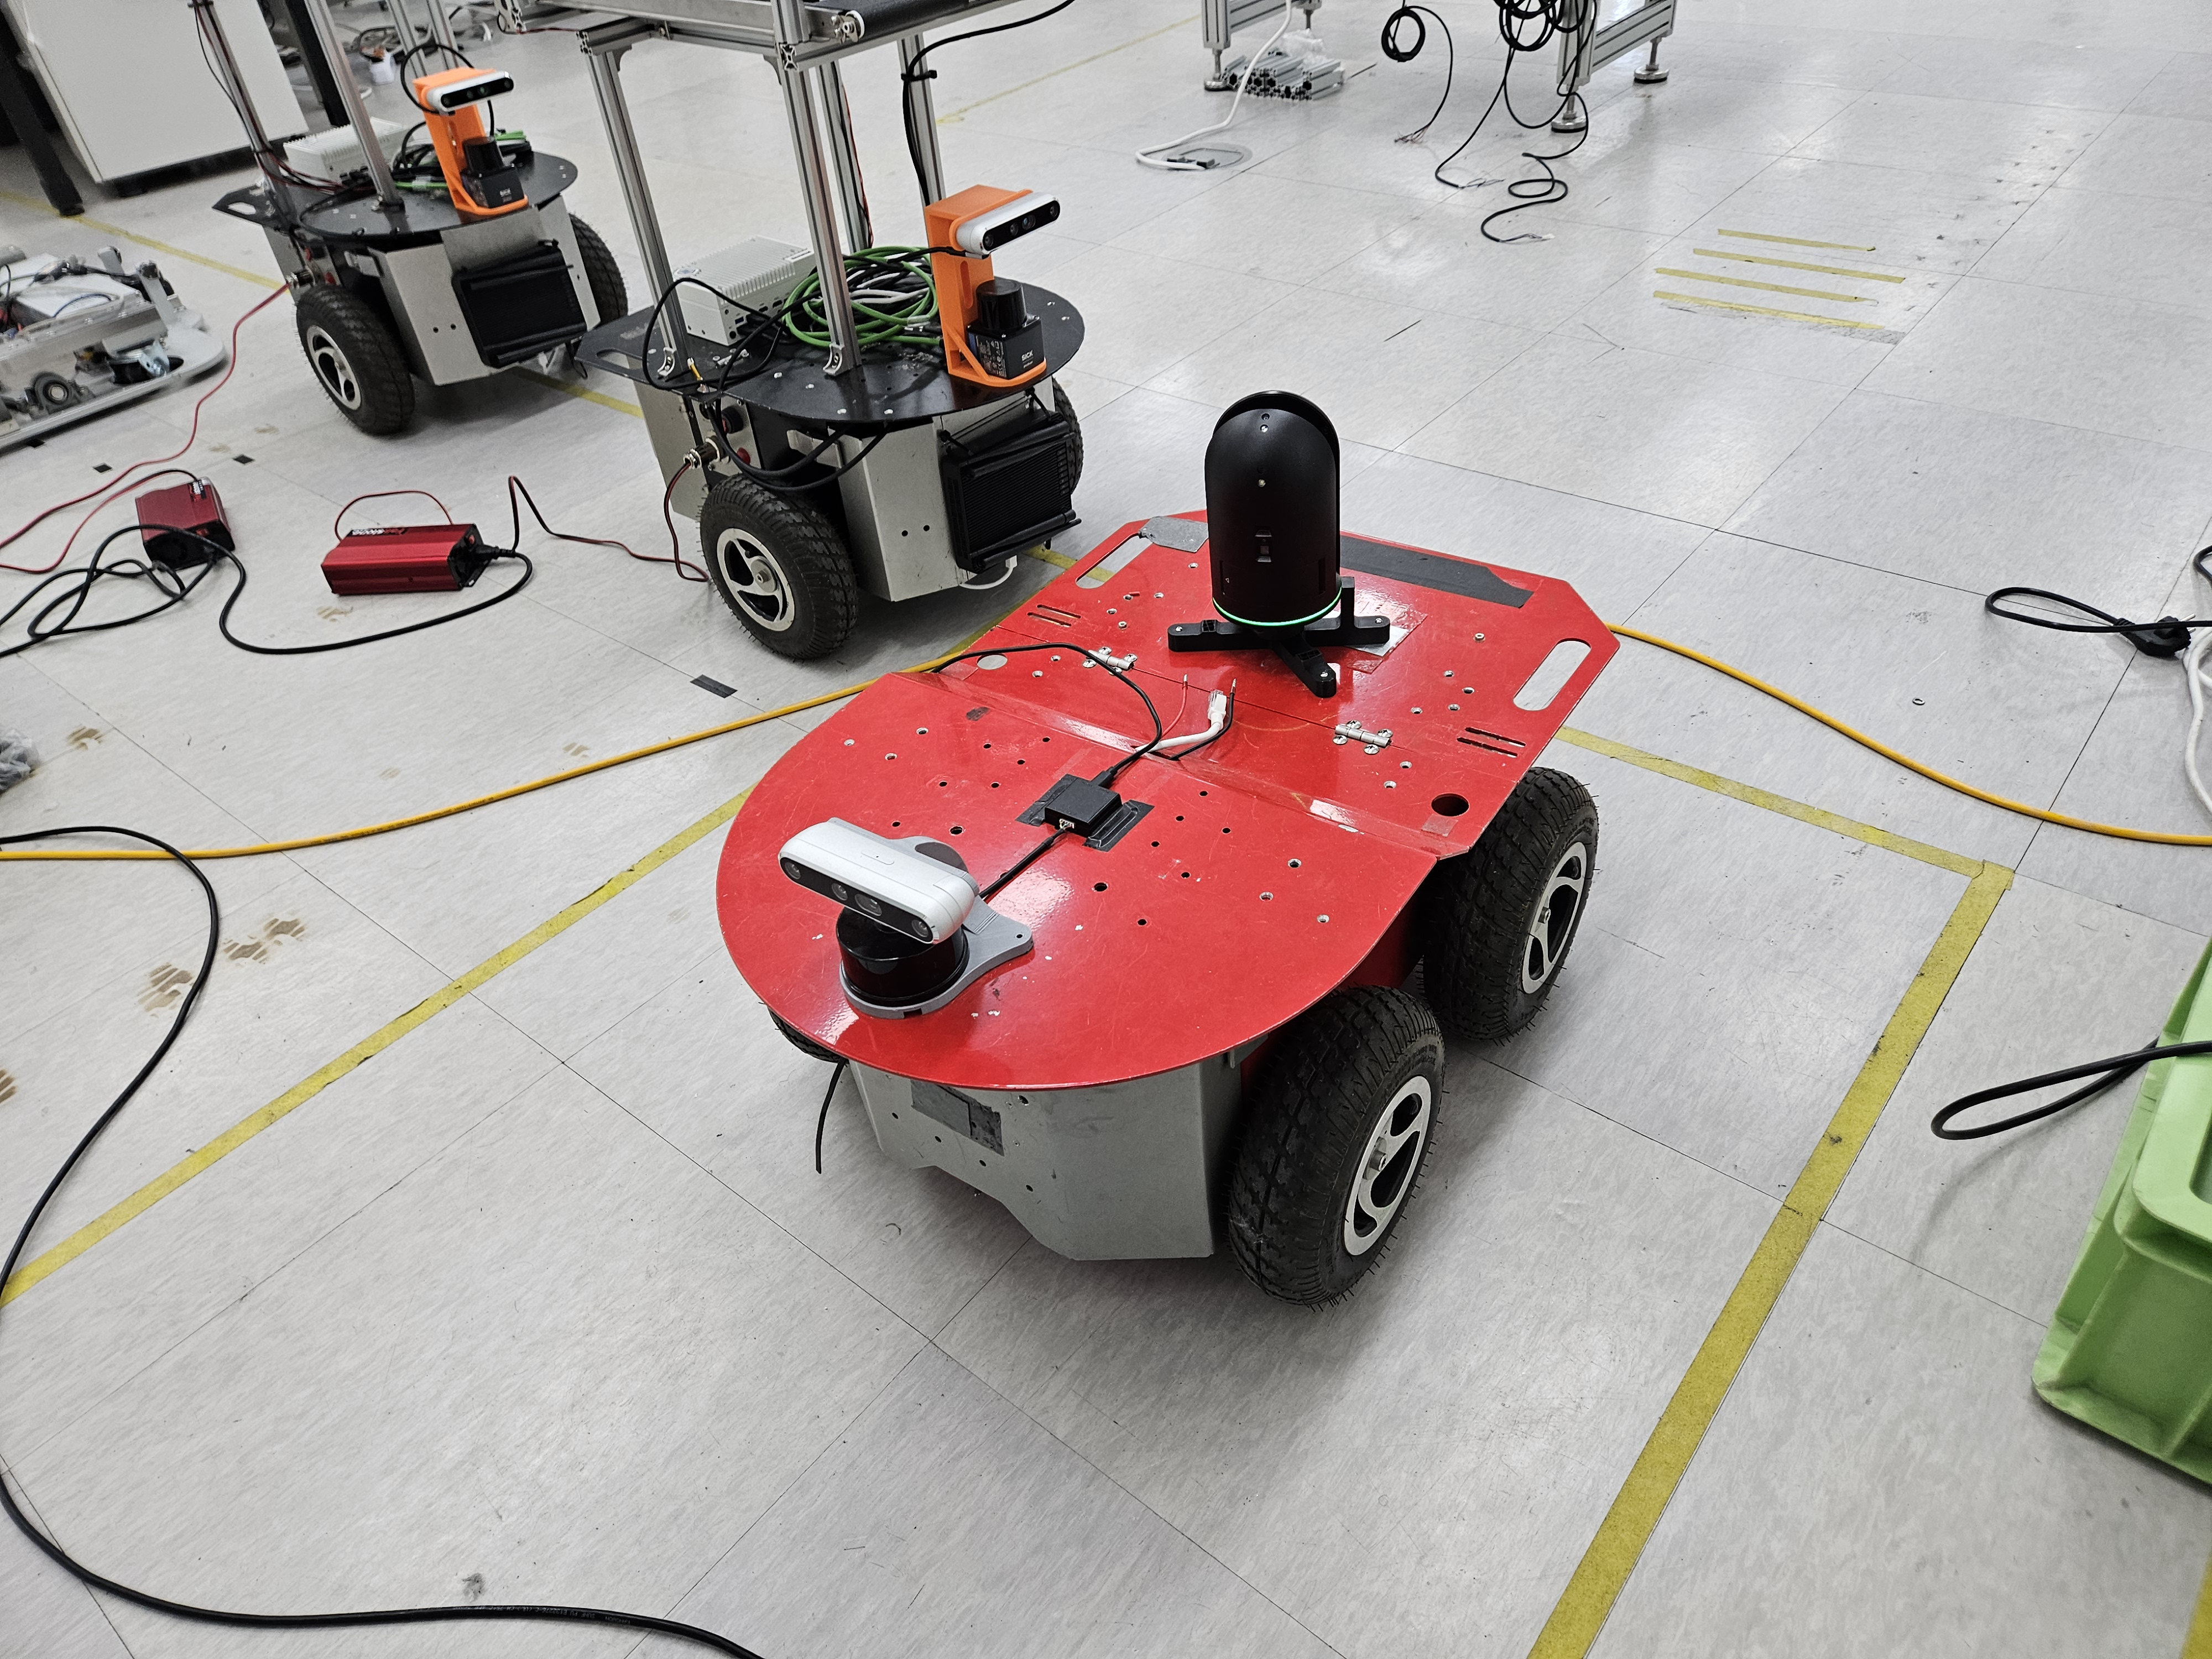
\includegraphics[width=0.82\linewidth]{figures/sen_fig13_redbot04_field.jpg}
\caption{RedBOT04 deployed in the industrial test room during the fully
autonomous on-hardware runs, with the Leica BLK360~G1 on its deck.}
\label{fig:field}
\end{figure}

The outcome reproduces the controlled ablation on the physical platform---a
platform kinematically and dimensionally different from the simulated
base---indicating that the effect is a property of the coverage model rather
than of any particular robot (Table~\ref{tab:fieldsim}, Figure~\ref{fig:fieldsim}).
The isotropic disk over-skips: it places only $1.8\pm0.5$ scans and, treating
floor behind the equipment island and furniture as covered, attains
$77.6\pm10.5\%$ LOS coverage with a large run-to-run variance, since whether
its few stations happen to see the occluded bays is largely incidental. The
visibility rule recognizes the occluded area as unseen, places $4.2\pm1.5$
scans, and covers $92.1\pm3.8\%$ of the free space reliably at the cost of
about two extra scans.

\begin{table}[htbp]
\centering
\caption{Fully autonomous on-hardware disk-versus-visibility comparison in the
physical test room ($N=4$ completed live runs per policy on RedBOT04; all
runs evaluated on the common reference map; mean~$\pm$~s.d.). Source:
\emph{Sensors}~\cite{kim2026sensors}.}
\label{tab:fieldsim}
\begin{tabular}{l c c}
\toprule
\textbf{Coverage model} & \textbf{Scans} & \textbf{LOS coverage (\%)} \\
\midrule
Isotropic disk (baseline)   & $1.8\pm0.5$ & $77.6\pm10.5$ \\
Ray-cast visibility (ours)  & $4.2\pm1.5$ & $\mathbf{92.1\pm3.8}$ \\
\bottomrule
\end{tabular}
\end{table}

\begin{figure}[!htb]
\centering
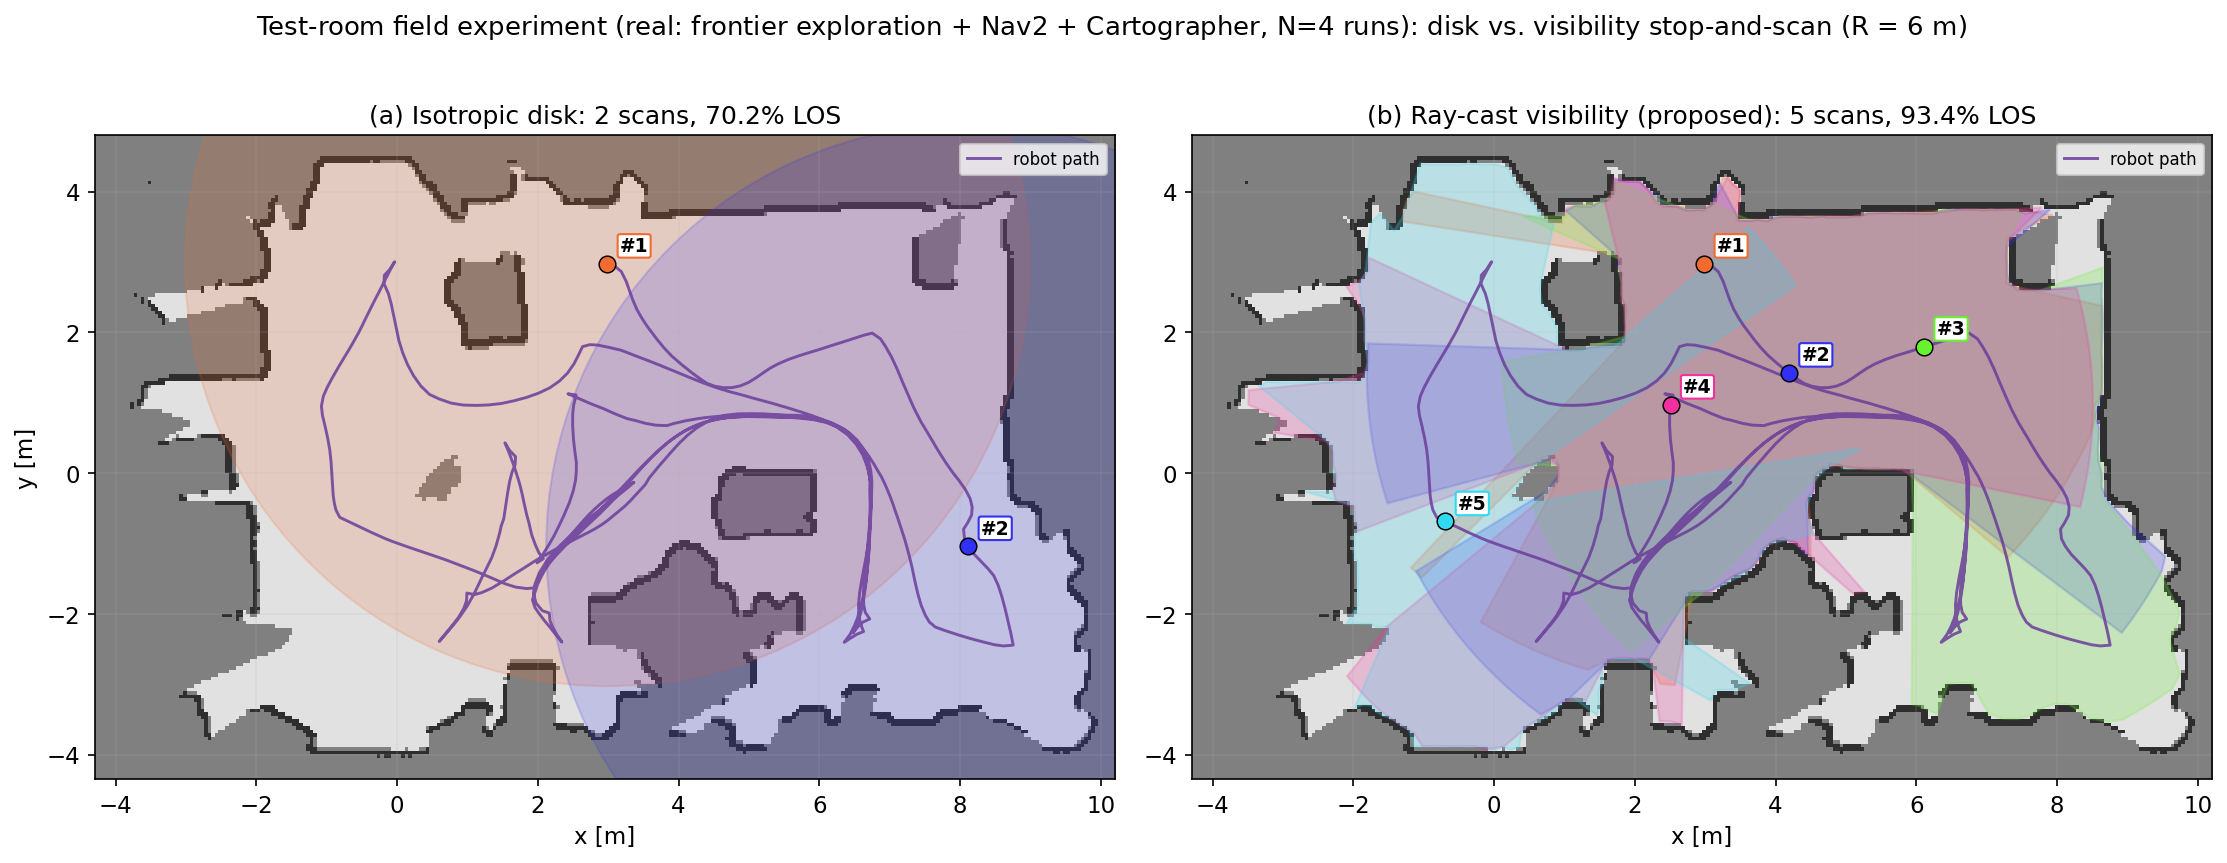
\includegraphics[width=\linewidth]{figures/sen_fig14_testroom_fieldsim.png}
\caption{Fully autonomous on-hardware comparison in the physical test room
(representative runs; $R=6$~m). Light gray: mapped free space; dark gray:
unmapped; black: occupied; purple line: autonomous robot path; colored
markers: placed scans with their coverage regions. (a)~Disk spacing rule;
(b)~visibility rule.}
\label{fig:fieldsim}
\end{figure}

\subsection{Survey-Grade Registration of the Autonomously Acquired Scans}
\label{subsec:exp-registration}

The remaining question is whether the scans each rule produces meet the
survey-grade premise. The BLK360 scans of every completed run were registered
offline, each run as an independent project under identical settings, in Leica
Cyclone REGISTER~360 PLUS using cloud-to-cloud alignment without artificial
targets (Table~\ref{tab:registration}). All four visibility runs registered at
survey grade: their networks comprise 3--6 setups joined by 3--13 pairwise
links, the bundle adjustments converged at 4--5~mm with overall overlaps of
84--88\%, and every individual link fell within the software's highest quality
band (per-link overlaps 74--92\%, errors 3--6~mm). The 4--5~mm bundle
residuals are of the same order as the scanner's stated single-setup accuracy.
The registered clouds reconstruct the room as a single coherent model
(Figures~\ref{fig:realreg} and~\ref{fig:regcloud}). The disk runs tell a
structurally different story: the three disk runs that placed two scans each
registered as a two-setup network with a single link (75--85\% overlap,
2~mm), and the fourth disk run placed only one scan and therefore admits no
registration at all. The low single-link residuals should not be read as
superior registration: with one link there is no redundancy, so the alignment
is not cross-checked by any independent constraint, and the resulting model
covers correspondingly less of the room. Bundle strengths are moderate
(38--48\%) across runs, reflecting the corridor-like traverses the explorer
takes; a loop-closing station layout, which the coverage-completion phase
naturally drives, would raise this redundancy measure.

\begin{table}[htbp]
\centering
\caption{Per-run offline registration of the autonomously acquired scans
(Leica Cyclone REGISTER~360 PLUS; cloud-to-cloud, no targets, identical
settings). Every link of every registered network lies within the software's
highest quality band (maximum error $\le15$~mm). Source:
\emph{Sensors}~\cite{kim2026sensors}.}
\label{tab:registration}
\begin{tabular}{l l c c c c}
\toprule
\textbf{Policy} & \textbf{Run} & \textbf{Setups} & \textbf{Links} & \textbf{Overall overlap (\%)} & \textbf{Bundle error (mm)} \\
\midrule
Visibility & 1 & 3 & 3  & 86 & 5 \\
Visibility & 2 & 6 & 13 & 86 & 5 \\
Visibility & 3 & 5 & 10 & 84 & 5 \\
Visibility & 4 & 3 & 3  & 88 & 4 \\
\midrule
Disk & 1 & 1 & 0 & \multicolumn{2}{c}{not registrable (single setup)} \\
Disk & 2 & 2 & 1 & 75 & 2 \\
Disk & 3 & 2 & 1 & 85 & 2 \\
Disk & 4 & 2 & 1 & 84 & 2 \\
\bottomrule
\end{tabular}
\end{table}

\begin{figure}[!htb]
\centering
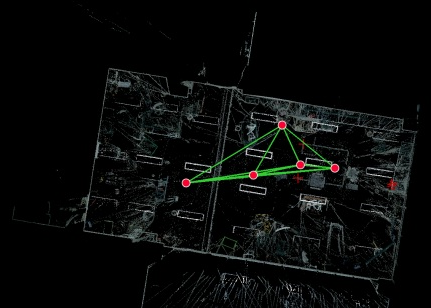
\includegraphics[height=5.0cm]{figures/sen_fig15_reg_network_vis.png}\hfill
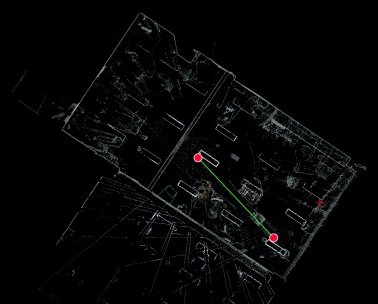
\includegraphics[height=5.0cm]{figures/sen_fig16_reg_network_disk.png}
\caption{Registered scan-station networks (top-down view; red markers are
setup positions, green edges are cloud-to-cloud links). (Left)~Visibility
run~3: five setups joined by ten redundant links reconstruct the room as a
single coherent model. (Right)~Disk run~4: two setups joined by a single
link---a minimal network with no redundant constraint.}
\label{fig:realreg}
\end{figure}

\begin{figure}[!htb]
\centering
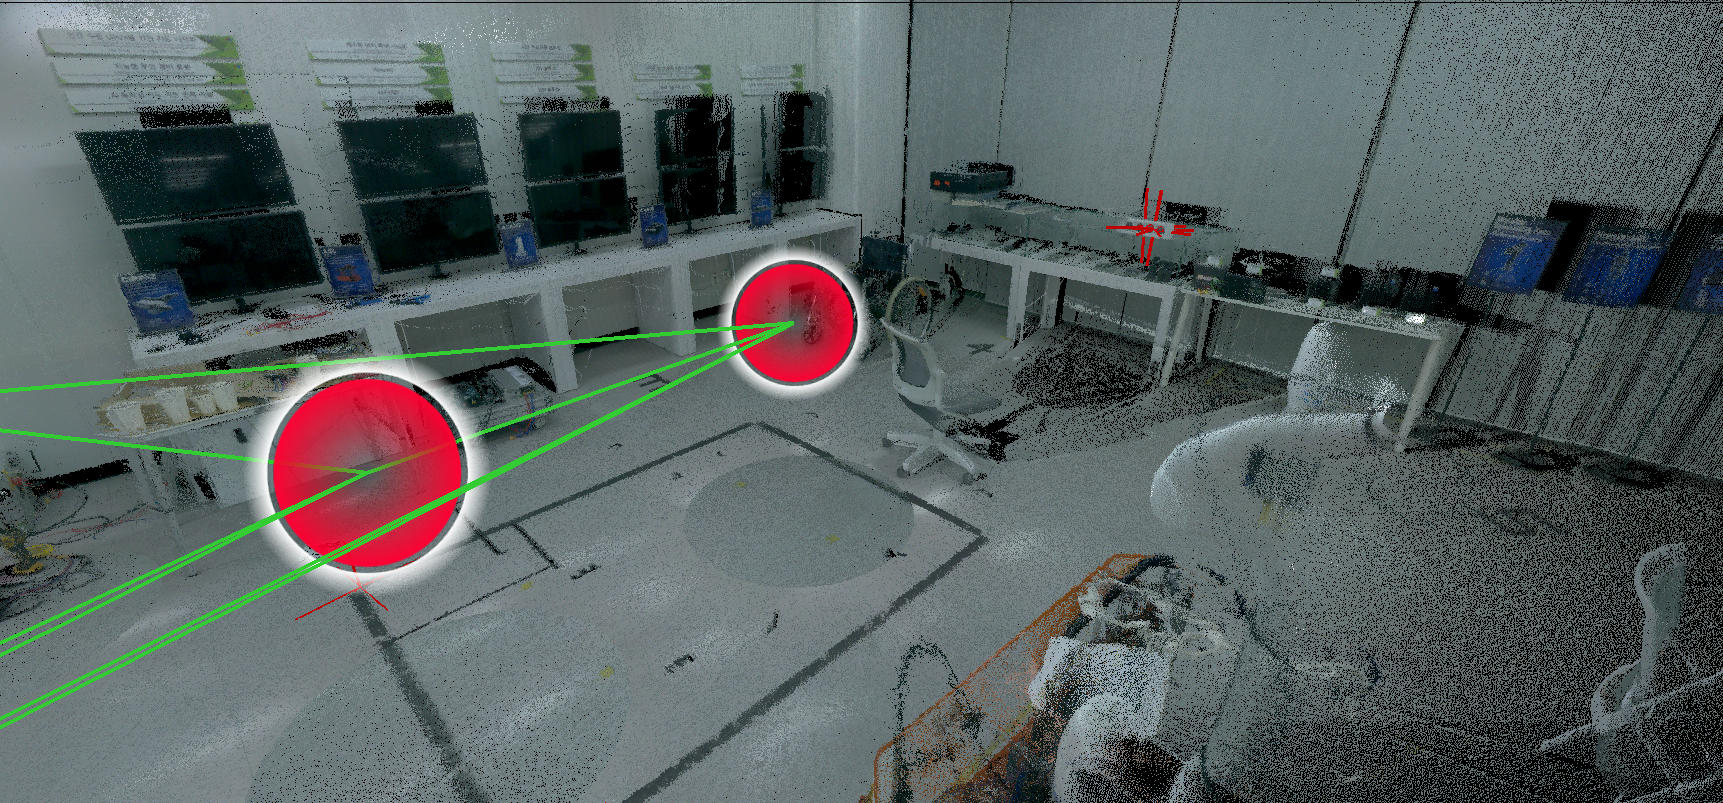
\includegraphics[width=0.49\linewidth]{figures/sen_fig17_regcloud_wall.png}\hfill
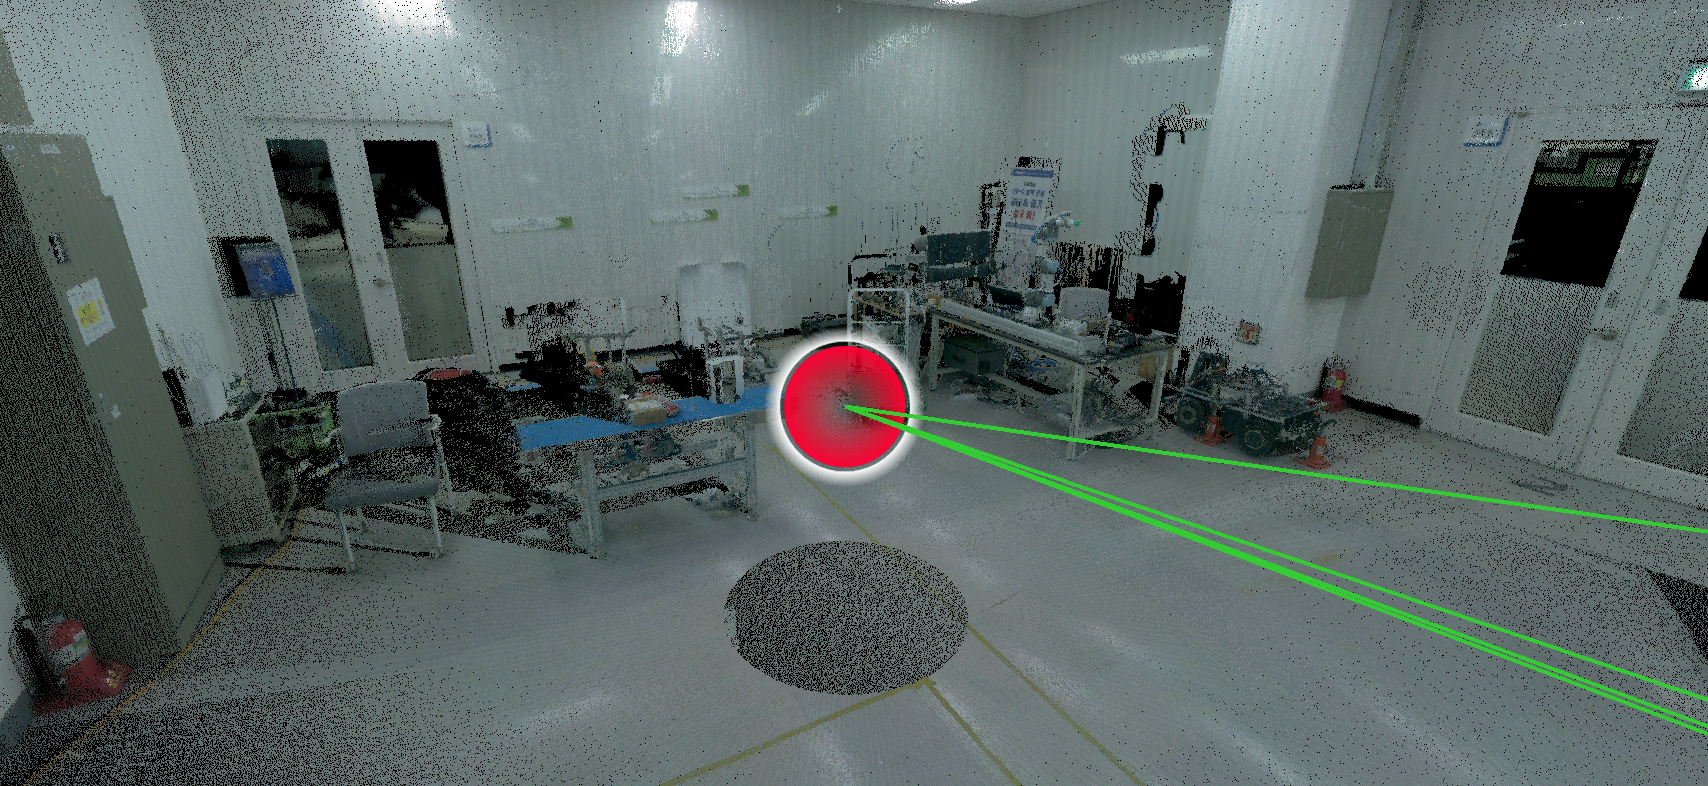
\includegraphics[width=0.49\linewidth]{figures/sen_fig18_regcloud_equipment.png}
\caption{Interior views of the registered colorized point cloud of visibility
run~3 along two diagonal directions: toward the display wall (left) and toward
the equipment side (right).}
\label{fig:regcloud}
\end{figure}

Together, the live comparison establishes that the visibility rule, not the
disk rule, reliably produces high-LOS scan placements, and the per-run
registration establishes that those placements consistently yield
survey-grade, bundle-verifiable scan networks, while disk placements do not
even guarantee a registrable network. The registered T2 and T3 clouds of
Table~\ref{tab:scenes} are the products of this subsystem that enter the
semantic modeling experiments below.

\section{Segmentation: Repeatability, Filtering, and Backbone Selection}
\label{sec:exp-seg}

\subsection{Backbone Selection against Learned Alternatives}
\label{subsec:exp-backbone}

The DBSCAN\,+\,Uni3D backbone was chosen against learned alternatives on a
wall-removed industrial scene of the test room (122.7~K points after
structural-plane removal; Figure~\ref{fig:nowallscene}). Because no point-level
ground truth exists for this scene, the metrics are deliberate screening
proxies: point \emph{coverage}, the fraction of input points assigned to some
object; the fraction of objects the open-vocabulary classifier cannot name
(\emph{unnameable}, a boundary-quality proxy because poor cuts produce more
unrecognizable fragments); and label diversity (Table~\ref{tab:backbones}).
For segmentation, the geometric clustering is compared against two
ScanNet-pretrained deep models, the superpoint-transformer instance segmenter
SPFormer~\cite{sun2023spformer} and the semantic-segmentation backbone Point
Transformer~V3~\cite{wu2024ptv3}, with every object subsequently named by the
same Uni3D classifier; for classification, Uni3D is compared against the
depth-projection classifier PointCLIP~V2~\cite{zhu2023pointclipv2}. Two further
instance segmenters, Mask3D~\cite{schult2023mask3d} and
Part2Object~\cite{shi2024part2object}, could not be evaluated because both
depend on a sparse-convolution backend incompatible with the experimental GPU.

\begin{figure}[!htb]
  \centering
  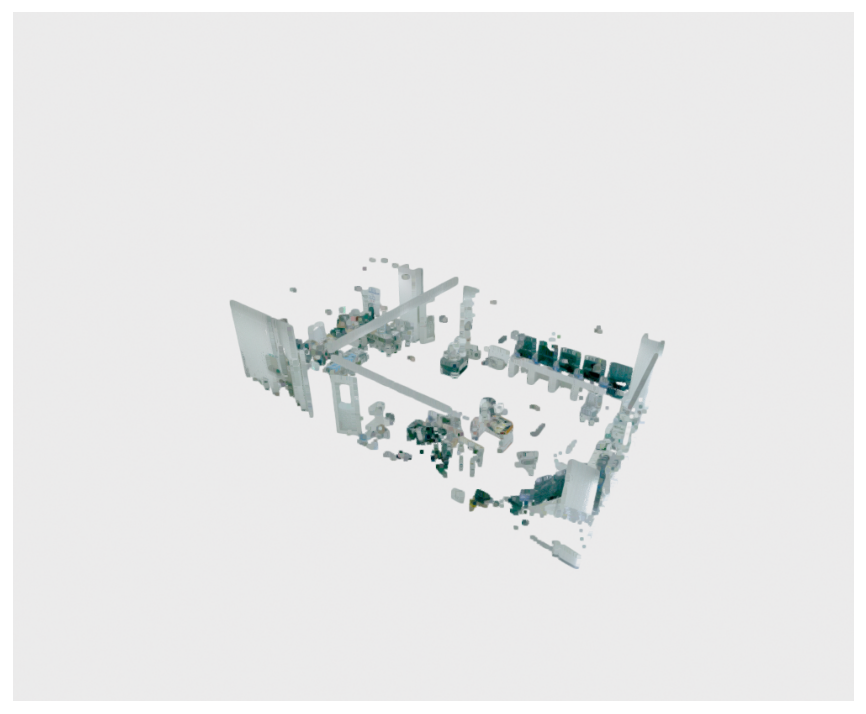
\includegraphics[width=0.7\textwidth]{figures/fig6_nowall.png}
  \caption{The backbone-selection scene: the test-room scan after
  structural-plane removal, shown in raw RGB (122{,}738 points). Only the
  object clutter remains, each connected cluster forming a candidate object.}
  \label{fig:nowallscene}
\end{figure}

\begin{table}[htbp]
\centering
\caption{Segmentation$\times$classification backbone comparison on the
wall-removed industrial scene (screening proxies; no point-level ground
truth). The PTv3 row is a semantic-segmentation head whose outputs are not
instance-comparable and is included only to document why closed-set semantic
heads were screened out.}
\label{tab:backbones}
\begin{tabularx}{\textwidth}{l c c c X}
\toprule
\textbf{Pipeline} & \textbf{Coverage} & \textbf{Unnameable} & \textbf{Classes} & \textbf{Dominant failure} \\
\midrule
\textbf{DBSCAN + Uni3D} & \textbf{98.3\%} & \textbf{23.3\%} & 13 & unlabeled coverage \\
SPFormer + Uni3D & 51.1\% & 45.9\% & 9 & furniture bias (chair 67/88) \\
PTv3 (semantic) & --- & --- & 17/20 emitted & 46\% ``wall'' after wall removal \\
DBSCAN + PointCLIP~V2 & 98.3\% & --- & 1--7 & collapse (pipe 23/30) \\
\bottomrule
\end{tabularx}
\end{table}

On every proxy, the geometric segmenter outperforms the deep closed-set model
on this out-of-distribution scene (Figure~\ref{fig:segcompare}). SPFormer
assigns only about half of the points to objects, because it fires only on
regions resembling its indoor-furniture training classes and lets genuine
industrial and robotic structure fall through; it over-segments the scene into
many partial or cross-object fragments that the classifier can no longer name,
and its label space is closed to eighteen indoor-furniture classes. PTv3 labels
46\% of all points \texttt{wall} on a scene from which the walls have already
been removed, and a further 20\% \texttt{refrigerator}: a closed-set per-point
model cannot abstain. PointCLIP~V2 collapses almost entirely to a single
category (\texttt{pipe} for 23 of 30 objects) at a deceptively high mean
confidence, because on the sparse, partial objects of a survey scan the depth
projections are too degenerate to be discriminative. The geometric backbone
wins not by being smarter but by refusing to guess: its failure mode is
unlabeled coverage, which the verification and owner layers are built to
absorb. Instance quality of the retained backbone is validated independently
below (owner-referenced sweep) and in Section~\ref{sec:exp-endtoend}
(end-to-end recall).

\begin{figure}[!htb]
  \centering
  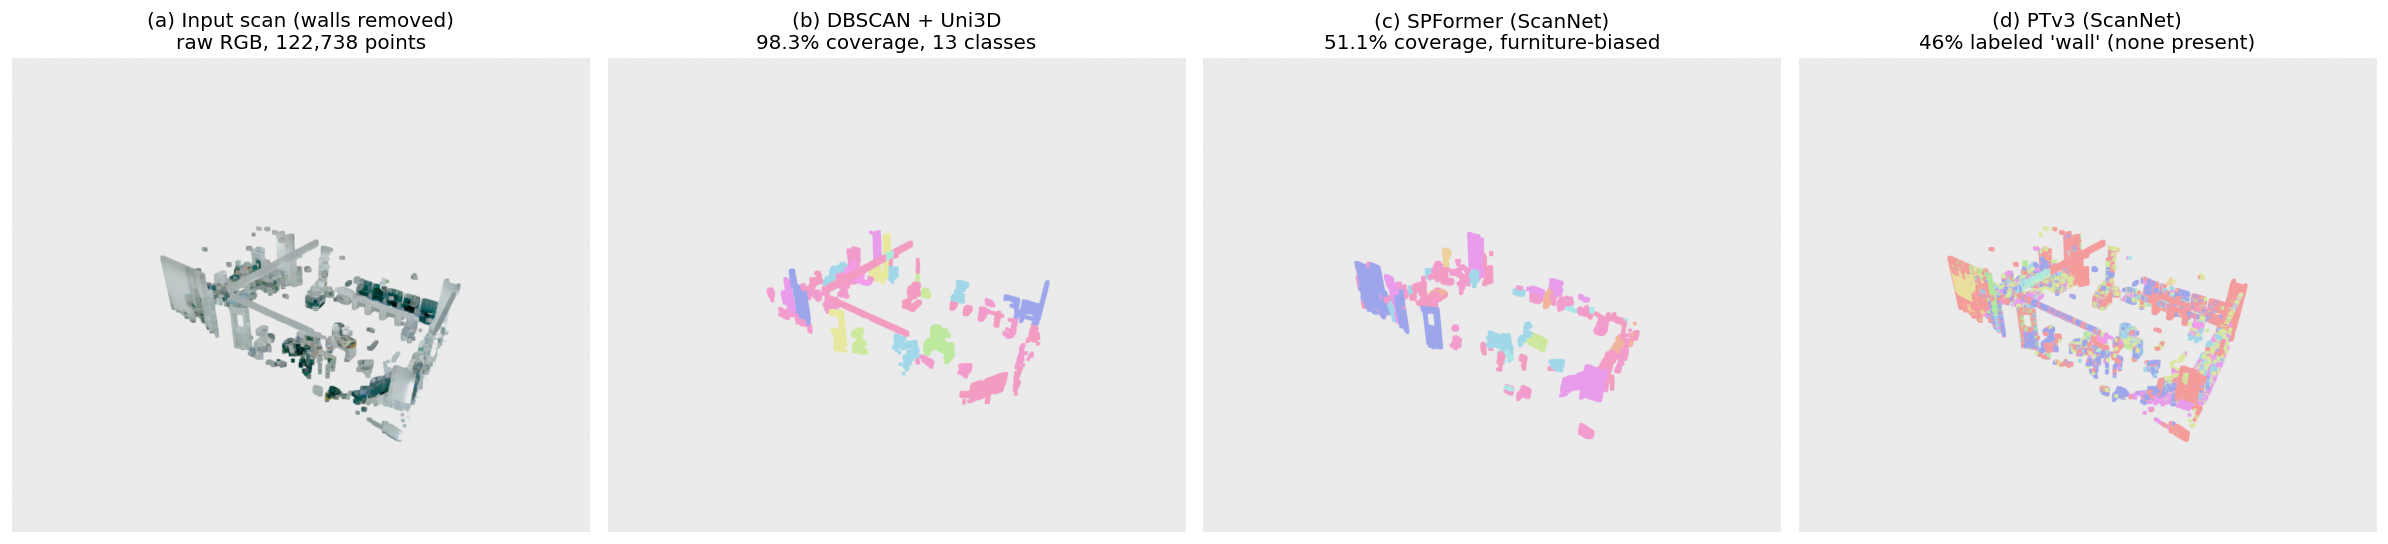
\includegraphics[width=\textwidth]{figures/fig6_2.png}
  \caption{Object segmentation on the test-room scan. (a)~The input cloud after
  wall removal (raw RGB). (b)--(d) are colored by predicted class: (b)~the
  geometric DBSCAN clustering with Uni3D labels covers the scene with coherent
  objects across 13 classes; (c)~SPFormer (ScanNet closed-set) assigns only
  about half of the points and biases toward indoor-furniture classes;
  (d)~PTv3 (ScanNet semantic) labels nearly half of the points \texttt{wall}
  although the walls were removed.}
  \label{fig:segcompare}
\end{figure}

\subsection{Repeatability and Remnant Filtering}
\label{subsec:exp-repeat}

Running the full pipeline twice from the same E57---including ten-plane
structure removal---reproduces every cluster byte-identically on both main
scenes (hash-verified). To probe robustness beyond one software stack, the
backbone was packaged into a version-pinned container and re-run under a
deliberately different environment (different glibc and Python patch
versions): all 81 retained robot-hall clusters remain byte-identical to the
native run. Running the same container on a second machine with a different
CPU vendor and microarchitecture (an Intel Core i9-13900H laptop versus the AMD
reference workstation) reproduces the identical per-cluster checksums---the
determinism claim holds across operating environments and x86-64 CPU vendors
under the pinned library set; bit-level reproducibility across instruction-set
architectures is not claimed. The structure-remnant filter of
Section~\ref{subsec:decomposition} removed all fourteen owner-confirmed
ceiling-soffit phantoms (seven per scene: showroom $45\rightarrow38$, robot
hall $88\rightarrow81$) while leaving every retained cluster unchanged. Before
the filter, these phantoms produced confidently verified fictions (keyboard
panels, handrails) that survived multi-view voting, since every view showed the
same wall-colored slab; detecting structure remnants geometrically, upstream of
semantics, proved more reliable than asking the verifier to doubt itself.

\subsection{Parameter Sensitivity and Coverage Stress}
\label{subsec:exp-params}

A 36-combination sweep (giant-split footprint $\times$ DBSCAN $\varepsilon$
$\times$ minimum points) shows a stable plateau at footprint 2.0--2.5~m:
instance recall degrades at 3.0~m as neighbors merge and at 1.5~m as equipment
shatters. Because scoring a sweep against the operating point's own
decomposition would be circular, every combination was re-scored against an
independent object-level reference: the owner-audited inventory in a
membership-independent form (all clean-cloud points falling inside each
owner-audited oriented box). On the robot hall (42 reference objects) the
min-points-100 band is a broad plateau and the operating point (2.5~m / 0.30 /
100) sits at the grid maximum (recall 0.952). On the showroom, the audit
surfaced an error, which is reported plainly: against the genuinely audited 57-object
inventory no grid combination of the base clustering exceeds recall 0.33---the
audited granularity of that scene is produced by the split-refinement stage,
not by any base-DBSCAN setting---so the parameter-robustness claim rests on the
non-circular robot-hall table. Two further perturbations bound the geometric
operating regime: voxel size is part of a jointly calibrated triple with
$(\varepsilon,\mathrm{min\_points})$ (at 3~cm the backbone recovers 42/42
reference objects, but 2~cm collapses recall to 0.36 as 22 objects merge and
5~cm to 0.33 as small objects starve), and seeded per-point Gaussian noise at
$\sigma=5$~mm---the scale of the scanner's real bundle error---drops recall to
0.48, with the 5~cm RANSAC inlier band saturating first. The T3 epoch supplied
a coverage stress case: at 99.6\% coverage, inter-object gaps close and DBSCAN
chains 120~K points (41\% of the clean cloud) into one $10.4\times9.6$~m
mega-cluster that survives the giant-split; refinement recovers little of the
resulting diff inflation, which is itself informative: about 88\% of that
epoch's absences reflect genuine scene change, not segmentation artifacts.

\subsection{Corrective Layers in Operation}
\label{subsec:exp-corrective}

Two T3 clusters that survived every upstream filter are \emph{diffuse webs}:
95~K and 13~K points spread over 80 and 12~m$^2$ at a 2D occupancy fill below
0.3, connected at $\sim$1.8~cm point spacing at any usable $\varepsilon$. The
diffuseness-gated re-split resolves them by \emph{cause} instead of size:
points hugging the exploration-grid wall line are structure noise ($\sim$70\%
of the 95~K-point residual), out-of-room bleed-through accounts for another 7\%,
and the remainder is re-clustered by occupancy-core erosion and split at the
support plane. The owner's ground truth for the largest compound---``a robot
arm on a desk, part of a mobile robot, wall noise''---is recovered exactly.
Applied to a 6.2~m wall-flush cluster that verification had confidently labeled
\texttt{electrical cabinet} (0.83), the wall-compound gate recovers the owner's
inventory at unit granularity: nine of the ten owner-confirmed monitor units,
the desk beneath them, and, from the off-wall remainder, a wheelchair robot;
unit boundaries are approximate because the dark screens return few points,
so the result is claimed as unit-level recall, not precise per-unit
segmentation. The structure-condition ensemble recovered two multi-meter
tables that exist in \emph{no} single-condition segmentation of the production
path---they appear only when walls are left in place---raising in-room recall
by four real objects ($\sim$8\%) as a standalone pass. The fusion also
quantifies label fragility: only 10 of 37 re-found objects keep the same label
across conditions, and cross-condition \emph{voting} corrected nothing, because
the verifier's biases are correlated across conditions (both recovered tables
were unanimously mis-verified as conveyor belts in every condition). Under a
pre-specified adoption rule, Point-SAM~\cite{zhou2024pointsam} separated 3/6
flagged merged clusters with sub-cluster labels reaching 9/11 versus 5/11 for
their parents, but automatic candidate selection also produced 2/6 false
positives, so it is retained only as an optional, manually triggered diagnostic
refinement (Figure~\ref{fig:baselines}).

\begin{figure}[!htb]
\centering
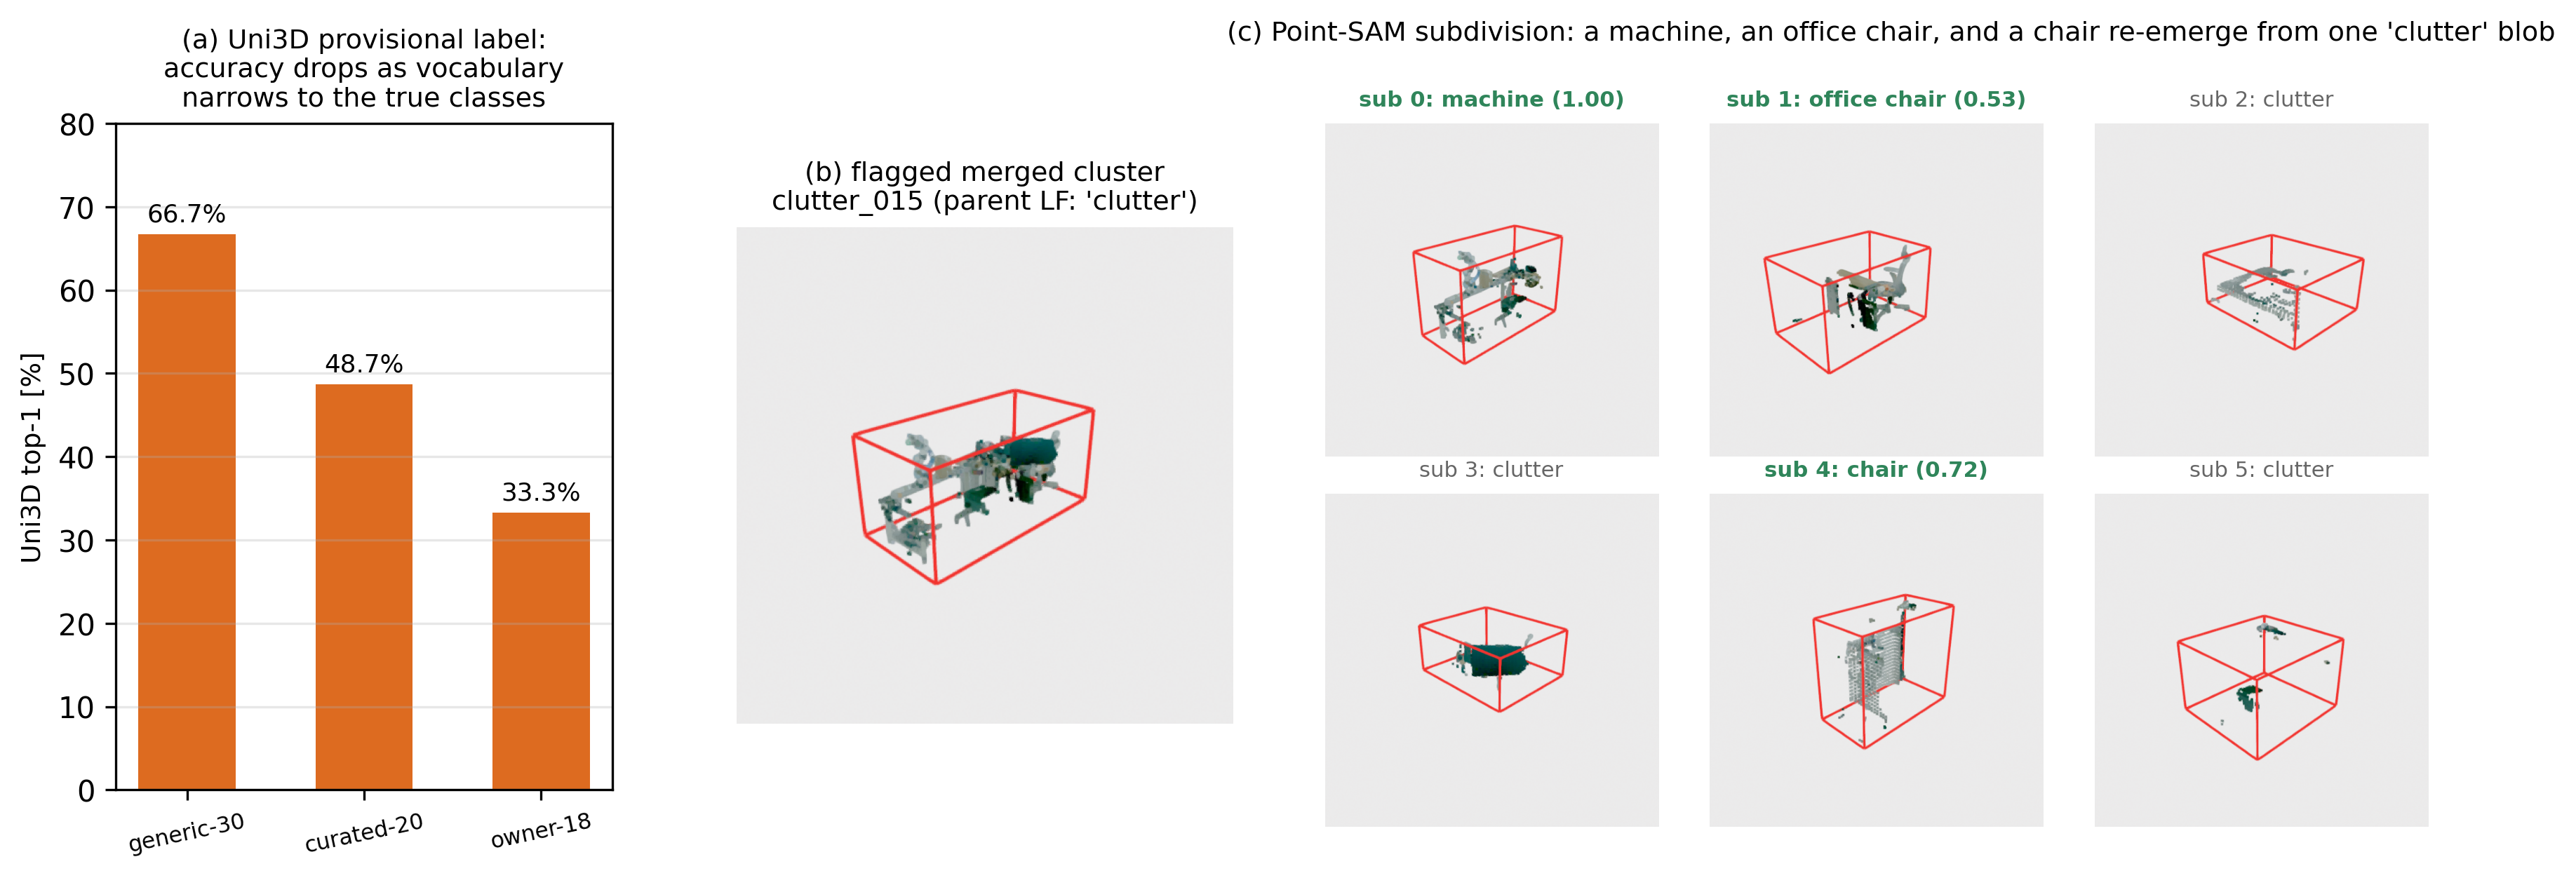
\includegraphics[width=0.95\linewidth]{figures/ele_fig13_pointsam_uni3d.png}
\caption{Learned components used as bounded tools. (a)~The Uni3D provisional
label degrades as the vocabulary narrows to the deployment's true classes
(Section~\ref{sec:exp-ablation})---why it is treated as untrusted context.
(b,c)~Conditional Point-SAM refinement of a flagged merged cluster: a machine,
an office chair, and a chair re-emerge from a single \texttt{clutter} blob,
each re-verified independently.}
\label{fig:baselines}
\end{figure}

\section{Verification: Multi-View Fusion and Escalation}
\label{sec:exp-verify}

\subsection{Multi-View Fusion Study}
\label{subsec:exp-multiview}

The first verification study, on the 57-object showroom decomposition, asks
how a VLM should consume multiple rendered views. Six configurations are
compared: a classifier-only reference, a $2\times2$ design over view count
(1 vs.\ 4, early fusion) and render/prompt generation (sparse renders with a
base prompt vs.\ dense renders with the guardrail prompt), and a sixth that
differs from four-view early fusion only in the fusion rule
(Table~\ref{tab:configs}). Labels are graded by two
independent references: a render audit by two of the authors against the dense
four-view renders and the measured dimensions, and the on-site inventory of the
facility operator by physical inspection, without reference to the render
audit. Audit-versus-inventory agreement is 79--95\% over the five VLM
configurations (Cohen's $\kappa$ 0.53--0.89). Three findings stand out
(Figure~\ref{fig:accuracy}).

\begin{table}[htbp]
\caption{Final type labels (57 showroom objects) under both references. Render
audit: C/P/W = correct / plausible / wrong, strict = C, lenient = C+P.
Inventory: strict matches on all 57 objects and on the 36 confirmed
non-structure objects. Source: ICTC~2026~\cite{kim2026ictc}.}
\label{tab:configs}
\centering
\begin{tabular}{l c c c c c c c}
\toprule
 & \multicolumn{5}{c}{\textbf{Render audit}} & \multicolumn{2}{c}{\textbf{Inventory}} \\
\textbf{Configuration} & C & P & W & strict & lenient & 57 & 36 \\
\midrule
Uni3D only (no VLM)            & 28 & 5  & 24 & 49\% & 58\% & 33 & 28 \\
1 view, base prompt, sparse    & 34 & 12 & 11 & 60\% & 81\% & \textbf{44} & \textbf{33} \\
4 views early fusion, sparse   & 28 & 10 & 19 & 49\% & 67\% & 34 & 27 \\
1 view, guardrails, dense      & 29 & 11 & 17 & 51\% & 70\% & 32 & 29 \\
4 views early fusion, dense    & 26 & 12 & 19 & 46\% & 67\% & 30 & 23 \\
4 views late fusion, dense     & 28 & \textbf{14} & \textbf{15} & 49\% & \textbf{74\%} & 34 & 28 \\
\bottomrule
\end{tabular}
\end{table}

\begin{figure}[!htb]
\centering
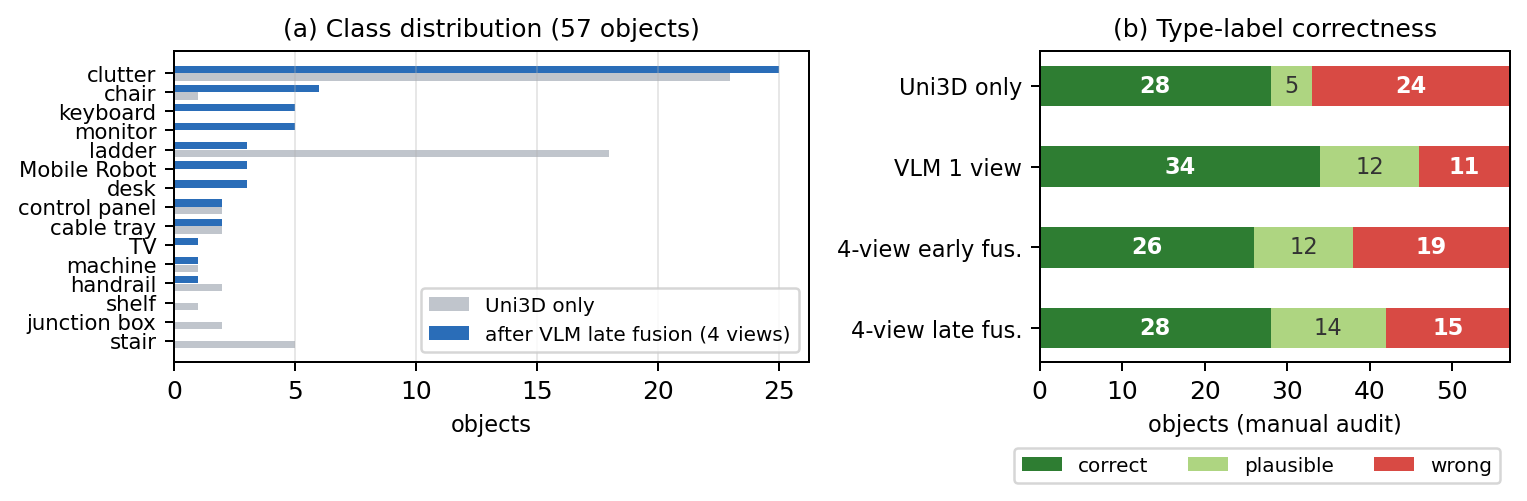
\includegraphics[width=0.95\linewidth]{figures/ictc_fig_accuracy.png}
\caption{Effect of VLM verification on the 57-object showroom scene.
(a)~Class distribution, classifier-only vs.\ after late fusion: implausible
\emph{ladder}/\emph{stair} populations are redistributed to displays and
furniture. (b)~Render audit: early fusion degrades single-view accuracy; late
fusion is the strongest multi-view strategy (15 wrong labels vs.\ 19 for
early fusion).}
\label{fig:accuracy}
\end{figure}

\emph{Early fusion hurts.} Feeding four sparse views into one prompt dropped
strict accuracy from 60\% (single view) to 49\%: extra oblique speckle views
encouraged over-committed readings, e.g., two electrical cabinets confidently
relabeled \emph{chair}; denser renders and the guardrails did not close the
gap, and the inventory confirms the direction. \emph{Late fusion is the
strongest multi-view strategy, but not the best configuration.} Judging each
view independently and voting beats early fusion on every measure (15 vs.\ 19
wrong labels, 74\% vs.\ 67\% lenient; 34 vs.\ 30 inventory matches) because a
contaminated view is outvoted, but it does not overtake the best single
canonical view (44/57 inventory matches, 77\%, versus 34/57): on sparse point
clouds extra views add noise faster than evidence, and the vote spends much of
its gain on caution. Late fusion is therefore claimed as the safer multi-view
rule, not as an accuracy gain over a well-chosen single view. \emph{Vote
unanimity is a free precision signal.} 17 of 57 objects received identical
labels from all four views; 16 of those (94\%) were audited correct and match
the inventory, versus 30\% (audit) or 18/40 (inventory) among split-vote
objects. Two re-runs of the late-fusion protocol bound the verifier's sampling
variance: accuracy on the 36 confirmed objects was 28, 27, and 27 across three
runs, and unanimity precision 16/17, 20/21, and 19/20 (94--95\%). Render
density produced the study's starkest warning: dense renders made four
dotted-grid panels look so convincingly like keyboards (per-view confidence up
to 0.97) that the label passed the render-based audit---only the inventory
revealed them to be ceiling-soffit remnants. A label that fools both the VLM
and a human at the same renders was still caught by vote splits, the strongest
argument for gating, and the incident motivated the structure-remnant filter.
On the late-fusion output, the implicit prompt marked 6 of 57 objects as key
objects (control panels, a large machine, mobile robots, and a wall display)
and 50 as movable; Figure~\ref{fig:ictccards} shows two completed records.

\begin{figure}[!htb]
\centering
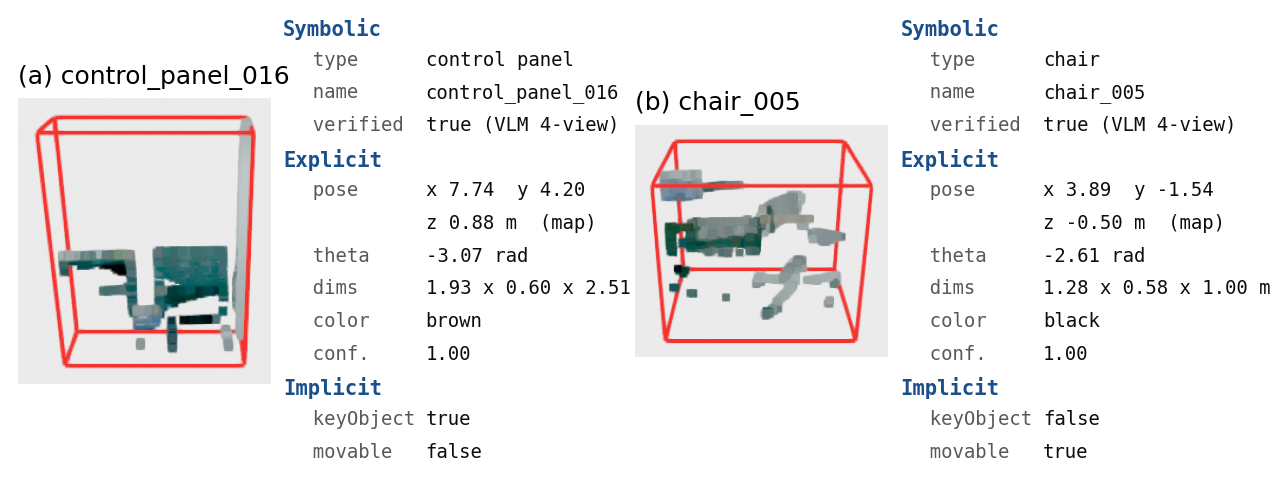
\includegraphics[width=0.95\linewidth]{figures/ictc_fig_cards.png}
\caption{Completed TOSM semantic-object records (dense render with symbolic /
explicit / implicit fields) as serialized into the VDA~5050-style message.
(a)~A control panel, unanimously verified and marked as a fixed key landmark.
(b)~An office chair corrected from \emph{stair}, movable and not a landmark.}
\label{fig:ictccards}
\end{figure}

\subsection{Escalation, Tiers, and Threshold Sensitivity}
\label{subsec:exp-escalation}

The escalation mechanism of Section~\ref{subsec:escalation} is evaluated on
both main scenes (Table~\ref{tab:verification}). Escalation lifts
confirmed-ground-truth accuracy from 77.8\% to 88.9\% on the showroom and from
78.1\% to 84.4\% on the robot hall (lenient: $76.2\%\rightarrow83.3\%$,
$n=42$), recovering 5 and 3 split-vote objects while regressing 1 and 0---a
consistent observed improvement across both scenes, though at these
sample sizes the paired contrast does not reach conventional significance
(exact McNemar $p=0.219$ and $p=0.25$), which the Wilson intervals make
explicit. Escalation adds 232 and 208 calls per scene at $\sim$\$0.009 per
call (Figure~\ref{fig:esccost}). The tier structure justifies the gating:
unanimous and escalated tiers reach 88.9--100\% precision, while the
unverified residue is 40--60\%---exactly the content the query interface must
demote. A repeat of the showroom run under identical settings bounds the
verifier's run-to-run variance at about $\pm3$ points. Verification yield
tracks scan quality: the manual scan leaves 47\% of objects unverified versus
24\% for exploration scans, and re-processing the T3 scan from a single setup
(1/6 coverage) drops the verified tier from 75.6\% to 56.6\% on identical
geometry---coverage buys verifiability, which ties Part~B back to Part~A.

\begin{table}[htbp]
\centering
\caption{Verification accuracy against confirmed ground truth, and per-tier
precision. Accuracy rows are over confirmed GT ($n=36$/32); trigger rates and
tier counts are over all GT-scored clusters (50 showroom / 51 robot hall).
Source: \emph{Electronics}~\cite{kim2026electronics}.}
\label{tab:verification}
\begin{tabular}{l c c c c}
\toprule
 & \multicolumn{2}{c}{\textbf{Showroom ($n=36$)}} & \multicolumn{2}{c}{\textbf{Robot hall ($n=32$)}} \\
 & base-4 & escalated & base-4 & escalated \\
\midrule
Accuracy & 77.8\% & \textbf{88.9\%} & 78.1\% & \textbf{84.4\%} \\
95\% Wilson CI & 61.9--88.3 & 74.7--95.6 & 61.2--89.0 & 68.2--93.1 \\
Recovered / regressed & \multicolumn{2}{c}{5 / 1} & \multicolumn{2}{c}{3 / 0} \\
Escalation trigger & \multicolumn{2}{c}{58\% (29/50)} & \multicolumn{2}{c}{51\% (26/51)} \\
\midrule
Unanimous precision & \multicolumn{2}{c}{100\% (19/19; 21 unan.)} & \multicolumn{2}{c}{94.4\% (17/18; 25 unan.)} \\
Escalated precision & \multicolumn{2}{c}{100\%} & \multicolumn{2}{c}{88.9\%} \\
Unverified precision & \multicolumn{2}{c}{60\%} & \multicolumn{2}{c}{40\%} \\
\bottomrule
\end{tabular}
\end{table}

\begin{figure}[!htb]
\centering
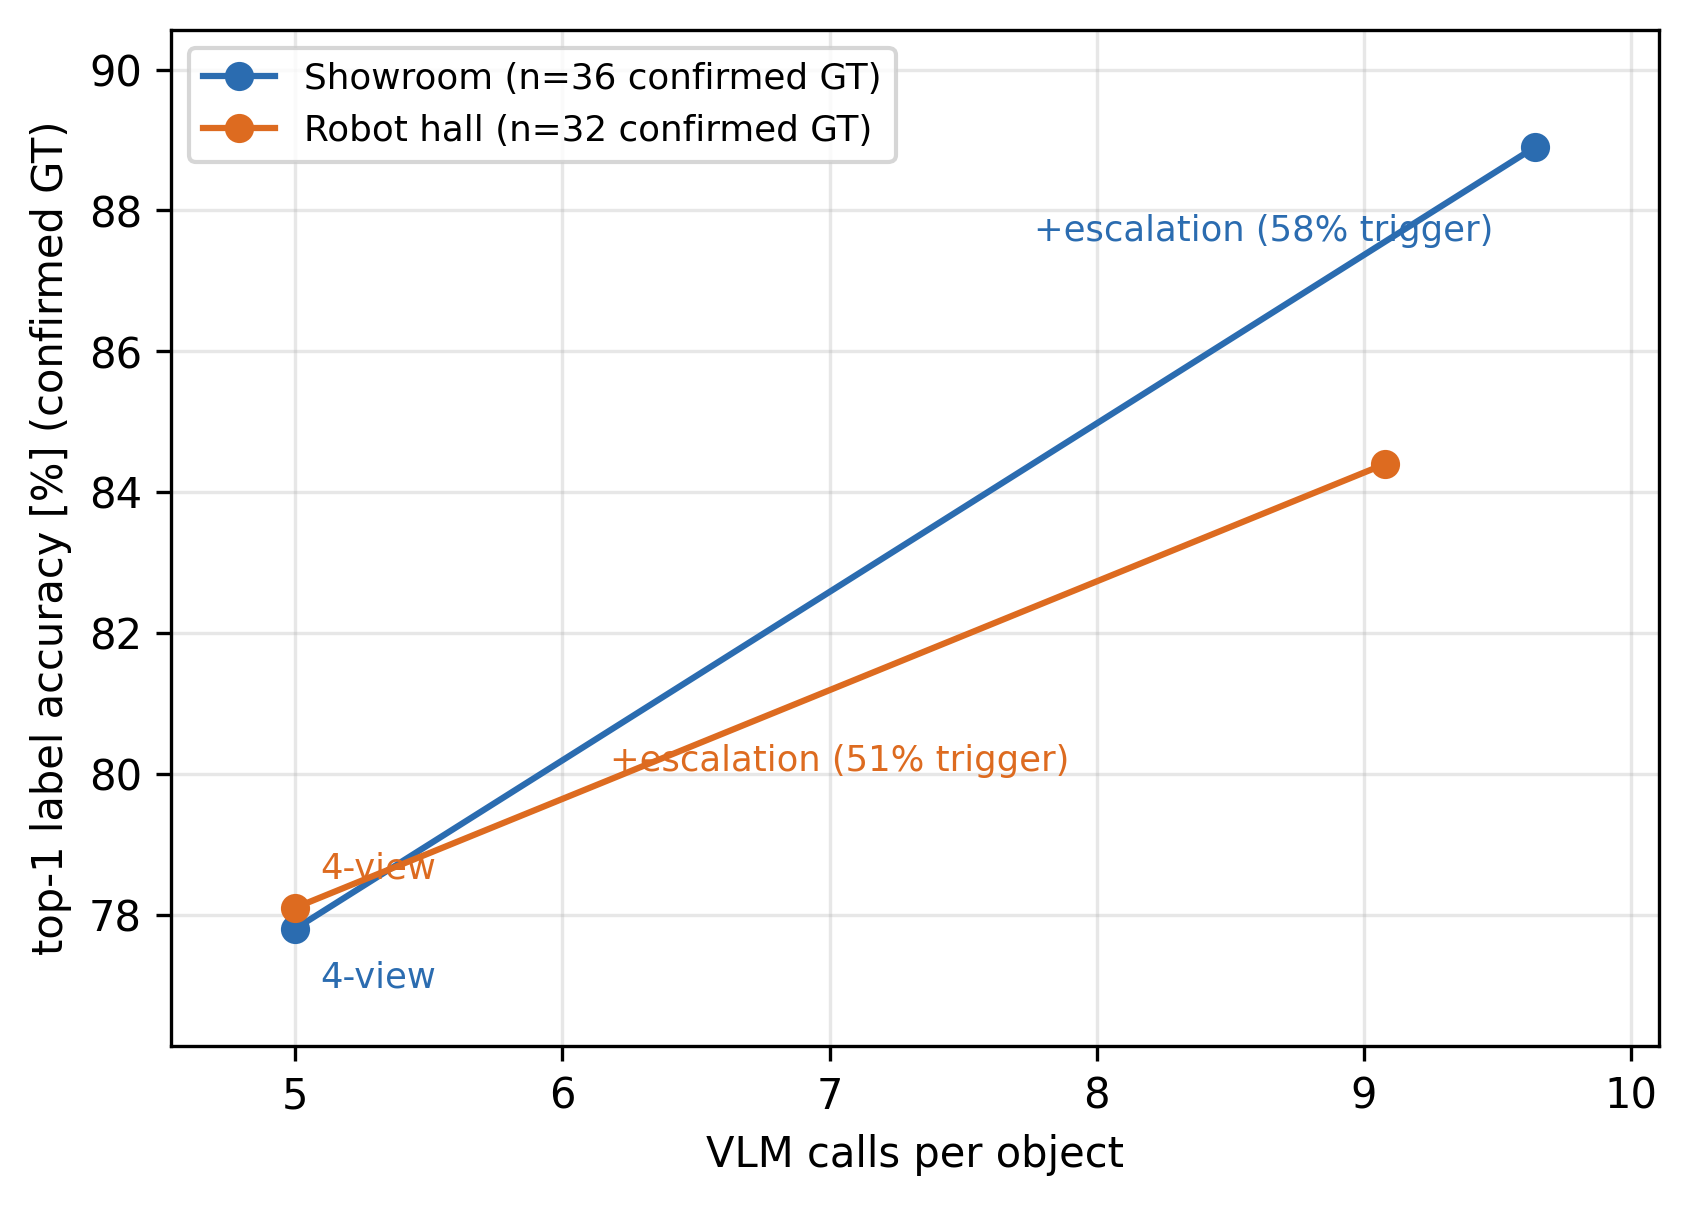
\includegraphics[width=0.85\linewidth]{figures/ele_fig6_escalation_cost.png}
\caption{Escalation accuracy--cost curves for both scenes.}
\label{fig:esccost}
\end{figure}

Precision alone understates what gating costs, so Table~\ref{tab:tierrf}
completes the tier picture with recall and $F_1$. The combined verified tier
reaches recall 0.722/0.781 on the two industrial scenes ($F_1$ 0.839/0.847)
but only 0.250 on the cafeteria, where the gate abstained on half of the
confirmed objects---the stress scene's segmentation failures surface as
recall, not as precision. Because the 0.6 share threshold gates status only,
its effect can be quantified exactly by re-scoring the stored votes at
alternative thresholds: sweeping 0.40--0.90 shows 0.6 sitting on a plateau
rather than a cliff, with $F_1$ maximized on a broad 0.45--0.65 band on both
industrial scenes and every 0.05 step moving at most one or two objects, so the
a priori 0.6 is retained rather than tuned post hoc.

\begin{table}[htbp]
\centering
\caption{Per-tier precision, recall, and $F_1$ on confirmed ground truth
(synonym-tolerant). The unverified row is the abstention tier.}
\label{tab:tierrf}
\small\setstretch{1.15}
\begin{tabular}{l l r r r r r}
\toprule
\textbf{Scene} & \textbf{Tier} & $n$ & $n_{\mathrm{conf}}$ & Prec. & Rec. & $F_1$ \\
\midrule
Showroom & verified (unanimous) & 21 & 19 & 1.000 & 0.528 & 0.691 \\
 & verified\_escalated & 8 & 7 & 1.000 & 0.194 & 0.326 \\
 & combined verified & 29 & 26 & 1.000 & 0.722 & 0.839 \\
 & unverified (abstained) & 21 & 10 & 0.600 & 0.167 & 0.261 \\
\midrule
Robot hall & verified (unanimous) & 25 & 18 & 0.944 & 0.531 & 0.680 \\
 & verified\_escalated & 16 & 9 & 0.889 & 0.250 & 0.390 \\
 & combined verified & 41 & 27 & 0.926 & 0.781 & 0.847 \\
 & unverified (abstained) & 10 & 5 & 0.400 & 0.062 & 0.108 \\
\midrule
Cafeteria & verified (unanimous) & 8 & 7 & 0.571 & 0.200 & 0.296 \\
 & verified\_escalated & 6 & 3 & 0.333 & 0.050 & 0.087 \\
 & combined verified & 14 & 10 & 0.500 & 0.250 & 0.333 \\
 & unverified (abstained) & 11 & 10 & 0.200 & 0.100 & 0.133 \\
\bottomrule
\end{tabular}
\end{table}

\subsection{Error Taxonomy and Class-Level Breakdown}
\label{subsec:exp-errors}

Four recurring error classes emerged (Figure~\ref{fig:taxonomy}):
(a)~\emph{structure-remnant phantoms}---soffit bands verified as keyboards,
eliminated upstream by the remnant filter; (b)~\emph{unanimous-but-wrong}---a
hanging chain unanimously verified as a door handle, partition fragments as
chairs, and at T3 a residual 7.4~m wall segment escalation-verified as a
staircase whose phantom label then propagated into a place name
(\texttt{staircase\_landing}), showing that place naming is verifier-bounded
too; a third case is the mirror image, in which the room's large wall-mounted
TV was geometrically detected yet left \texttt{unverified} while a small
co-located cluster was verified as a fire extinguisher the owner refuted;
(c)~\emph{clutter absorption}---a disassembled robot, a poster stand, and a
low-reflectance floor fan (674 points) each unanimously verified as
\texttt{clutter}: geometrically detected, semantically flattened; and
(d)~\emph{render ambiguity} $\rightarrow$ \texttt{unverified}, the intended
failure mode. Classes (b) and (c) motivate reporting verification as tiered
evidence rather than truth. Table~\ref{tab:classdist} disaggregates every
scene's ground truth into class families: robots are the worst family
everywhere they occur (0/4, 0/3, and 0/8 correct across the three
robot-bearing sets)---absorption, not misperception, since most land in
\texttt{clutter} or abstain---and displays and fixtures abstain heavily on the
showroom, exactly the render-ambiguous shapes the taxonomy predicts.

\begin{figure}[!htb]
\centering
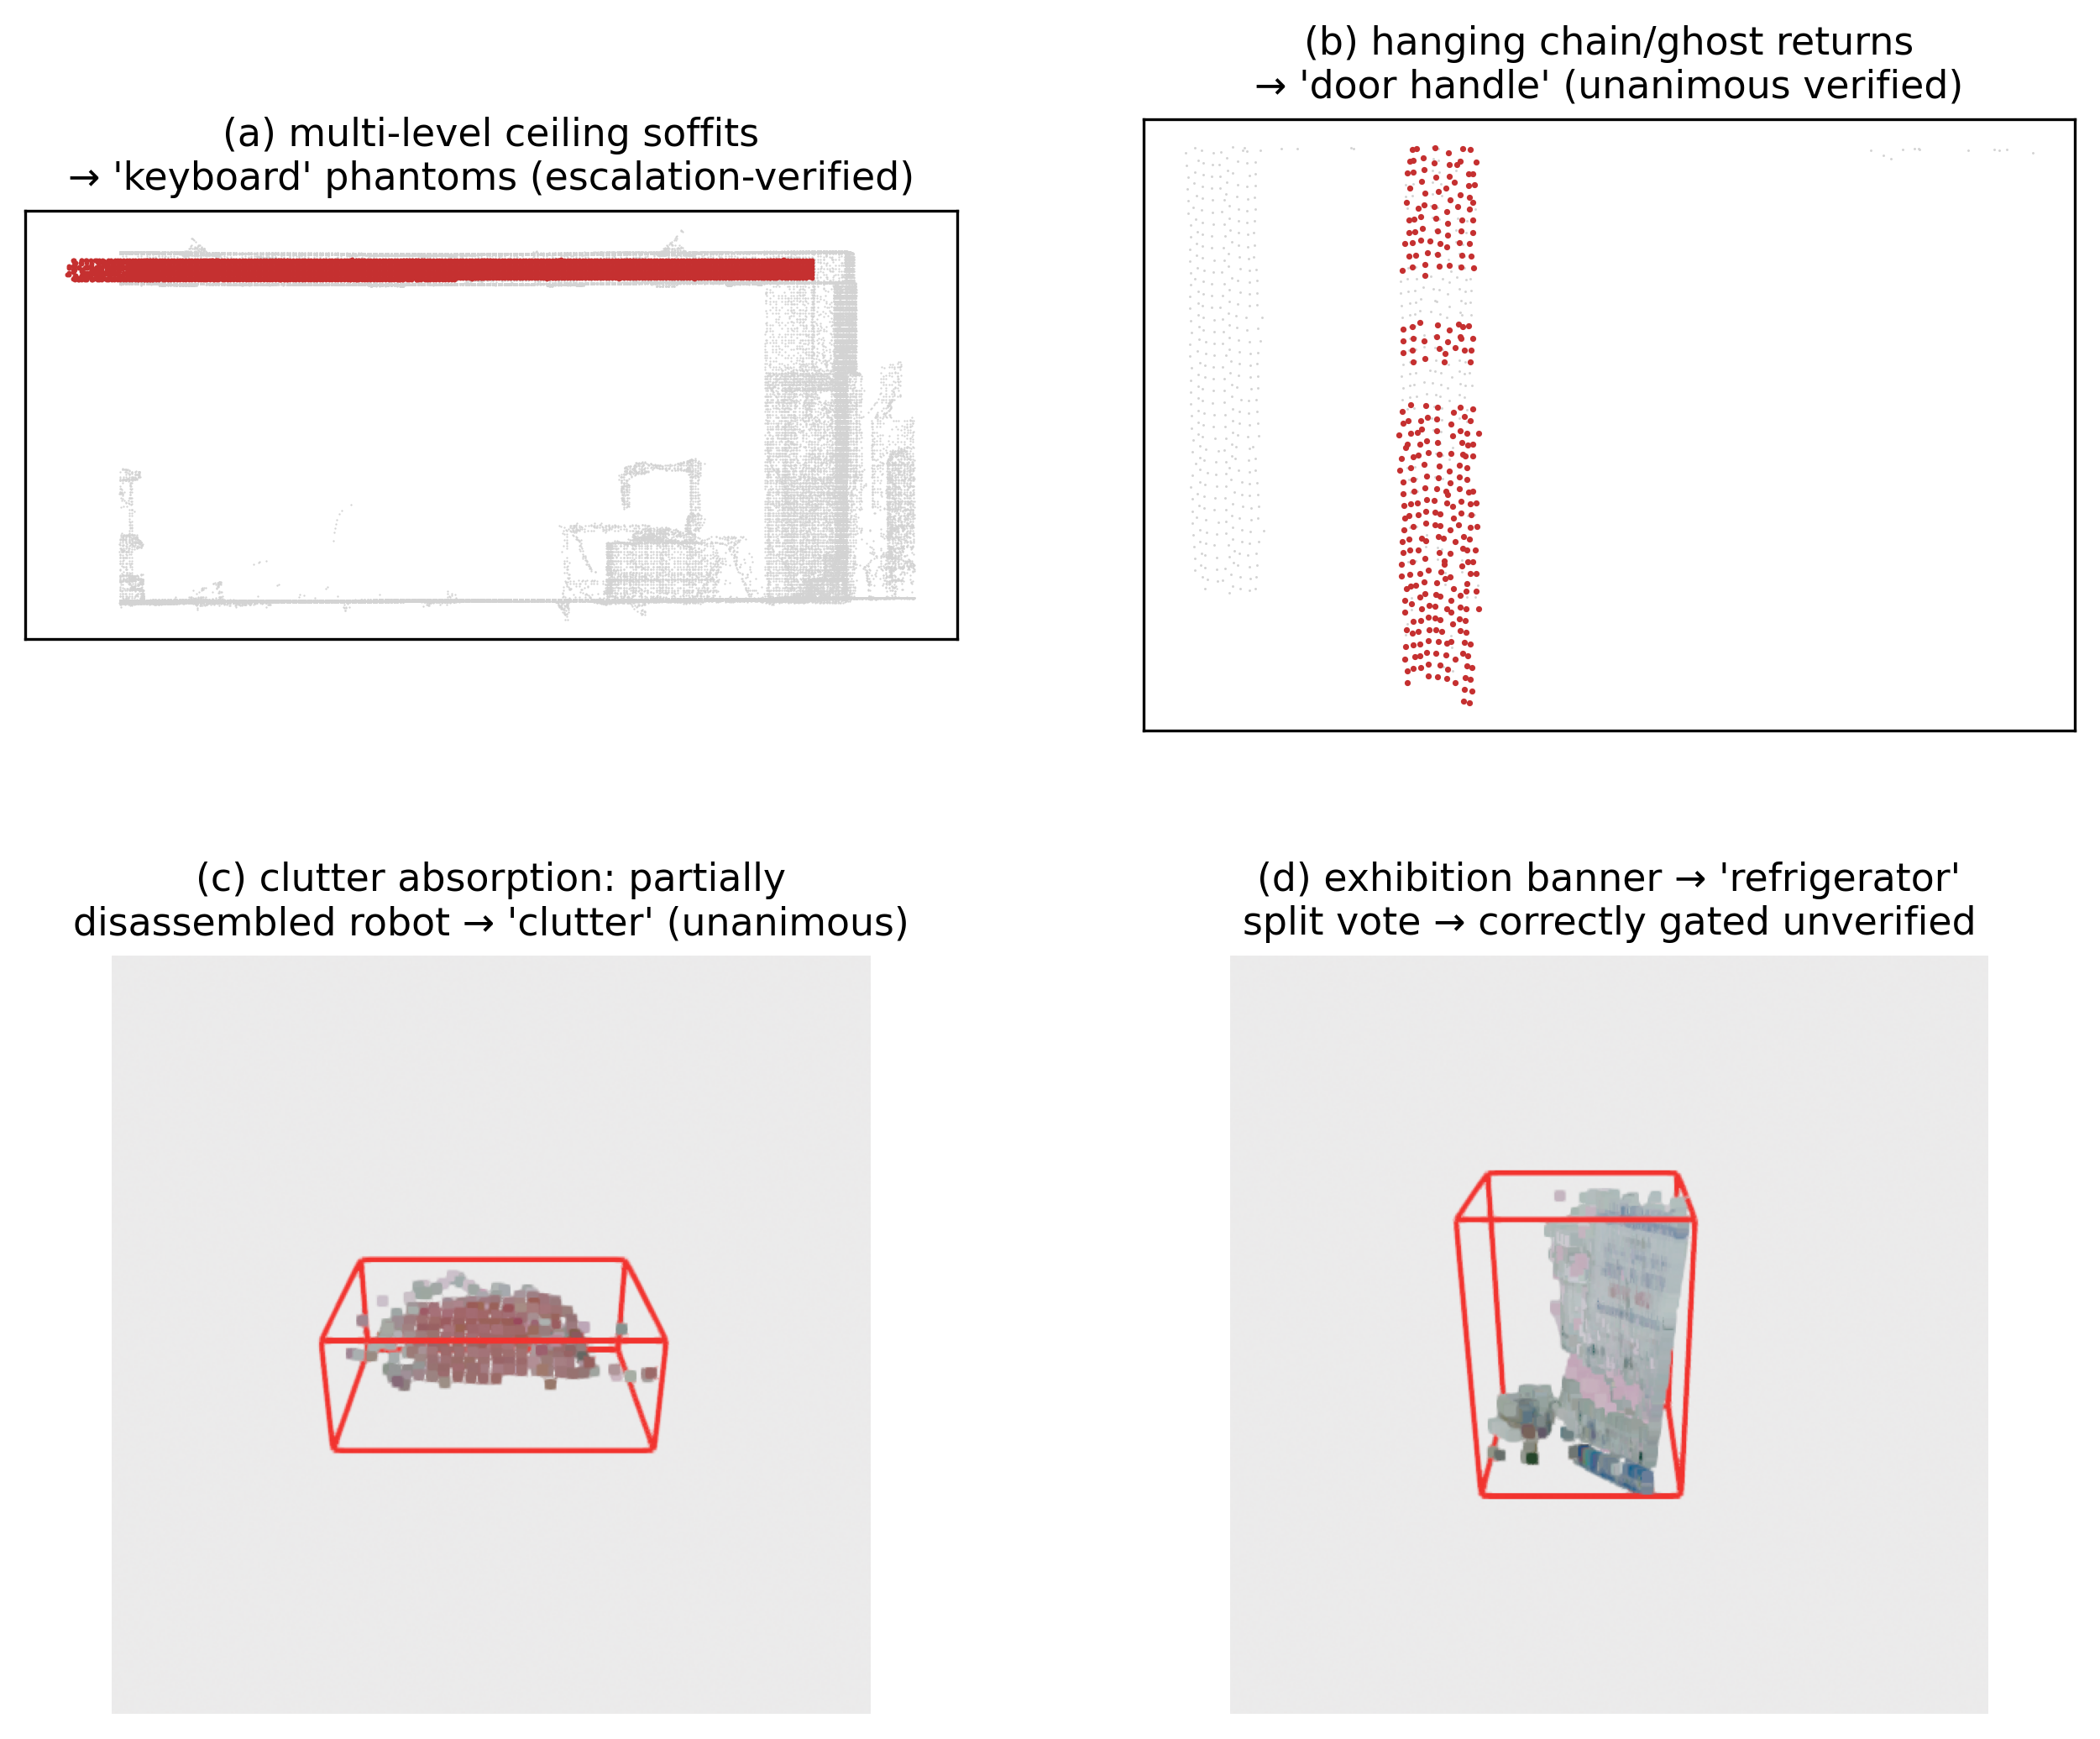
\includegraphics[width=0.9\linewidth]{figures/ele_fig10_error_taxonomy.png}
\caption{Verification error taxonomy: remnant phantom, unanimous-but-wrong,
clutter absorption, render ambiguity.}
\label{fig:taxonomy}
\end{figure}

\begin{table}[htbp]
\centering
\caption{Ground-truth object classes per scene, grouped into families, with
each object's verification outcome in the canonical run. ``Filtered'' =
excluded before scoring (structure artifact or out of room scope).}
\label{tab:classdist}
\small\setstretch{1.15}
\begin{tabular}{l l r r r r r}
\toprule
\textbf{Scene} & \textbf{Family} & GT & Corr. & Wrong & Unver. & Filt. \\
\midrule
Showroom (57-set) & seating & 5 & 4 & 1 & 0 & 0 \\
 & robots & 4 & 0 & 1 & 3 & 0 \\
 & displays/monitors & 5 & 0 & 0 & 5 & 0 \\
 & machines/electrical & 6 & 3 & 0 & 3 & 0 \\
 & furniture & 2 & 0 & 0 & 2 & 0 \\
 & fixtures & 6 & 0 & 0 & 6 & 0 \\
 & structure-noise & 7 & 0 & 0 & 0 & 7 \\
 & clutter/unknown & 22 & 20 & 0 & 2 & 0 \\
 & \emph{total} & 57 & 27 & 2 & 21 & 7 \\
\midrule
Robot hall (det) & seating & 5 & 4 & 0 & 1 & 0 \\
 & robots & 3 & 0 & 1 & 2 & 0 \\
 & displays/monitors & 1 & 0 & 0 & 0 & 1 \\
 & machines/electrical & 1 & 0 & 0 & 0 & 1 \\
 & furniture & 2 & 0 & 0 & 0 & 2 \\
 & fixtures & 8 & 3 & 1 & 4 & 0 \\
 & structure-noise & 8 & 0 & 0 & 1 & 7 \\
 & clutter/unknown & 53 & 25 & 7 & 2 & 19 \\
 & \emph{total} & 81 & 32 & 9 & 10 & 30 \\
\midrule
Cafeteria & seating & 10 & 1 & 4 & 5 & 0 \\
 & machines/electrical & 1 & 1 & 0 & 0 & 0 \\
 & furniture & 1 & 0 & 1 & 0 & 0 \\
 & fixtures & 5 & 0 & 1 & 4 & 0 \\
 & structure-noise & 3 & 0 & 0 & 0 & 3 \\
 & clutter/unknown & 8 & 4 & 2 & 2 & 0 \\
 & \emph{total} & 28 & 6 & 8 & 11 & 3 \\
\midrule
T3 re-scan (owner GT) & seating & 5 & 2 & 2 & 1 & 0 \\
 & robots & 8 & 0 & 6 & 2 & 0 \\
 & displays/monitors & 2 & 0 & 1 & 1 & 0 \\
 & machines/electrical & 4 & 0 & 4 & 0 & 0 \\
 & furniture & 4 & 0 & 3 & 1 & 0 \\
 & fixtures & 4 & 0 & 2 & 2 & 0 \\
 & structure-noise & 9 & 0 & 6 & 3 & 0 \\
 & clutter/unknown & 5 & 4 & 0 & 0 & 0 \\
 & \emph{total} & 41 & 6 & 25 & 10 & 0 \\
\bottomrule
\end{tabular}
\end{table}
